\chapter{焦点面検出器アライメントの較正}
\label{chapter4}

GroundBIRD実験での偏光測定のためには、検出器間での信号の差分を取ることが重要であり、それに伴って望遠鏡のスキャンに対して最適な検出器のアライメントが求められる。この章では検出器アライメントの最適化に向けた改善を行い、観測データからその効果を確認した。

\section{検出器アライメントの問題点}

\subsection{スキャン軸に対する傾きと差分解析}
まず、GroundBIRDでの解析手法の1つである差分解析と検出器アライメントの関係について述べる。\ref{mkid_design}で示したように、焦点面検出器は異なる偏光方向に感度を持った検出器が交互に配置されている。これらの検出器が検出する信号は空のある点からの放射が望遠鏡内の光学系を経て焦点面へと届いたものである。つまり、焦点面での検出器の配置を空へと射影した時にどう配置されているかが重要になる。各検出器は空のある点を見ており、望遠鏡の方位角回転に伴って同じ仰角の空を回転しながら観測する(図\ref{scan_image})。
\begin{figure}[htbp]
  \centering
  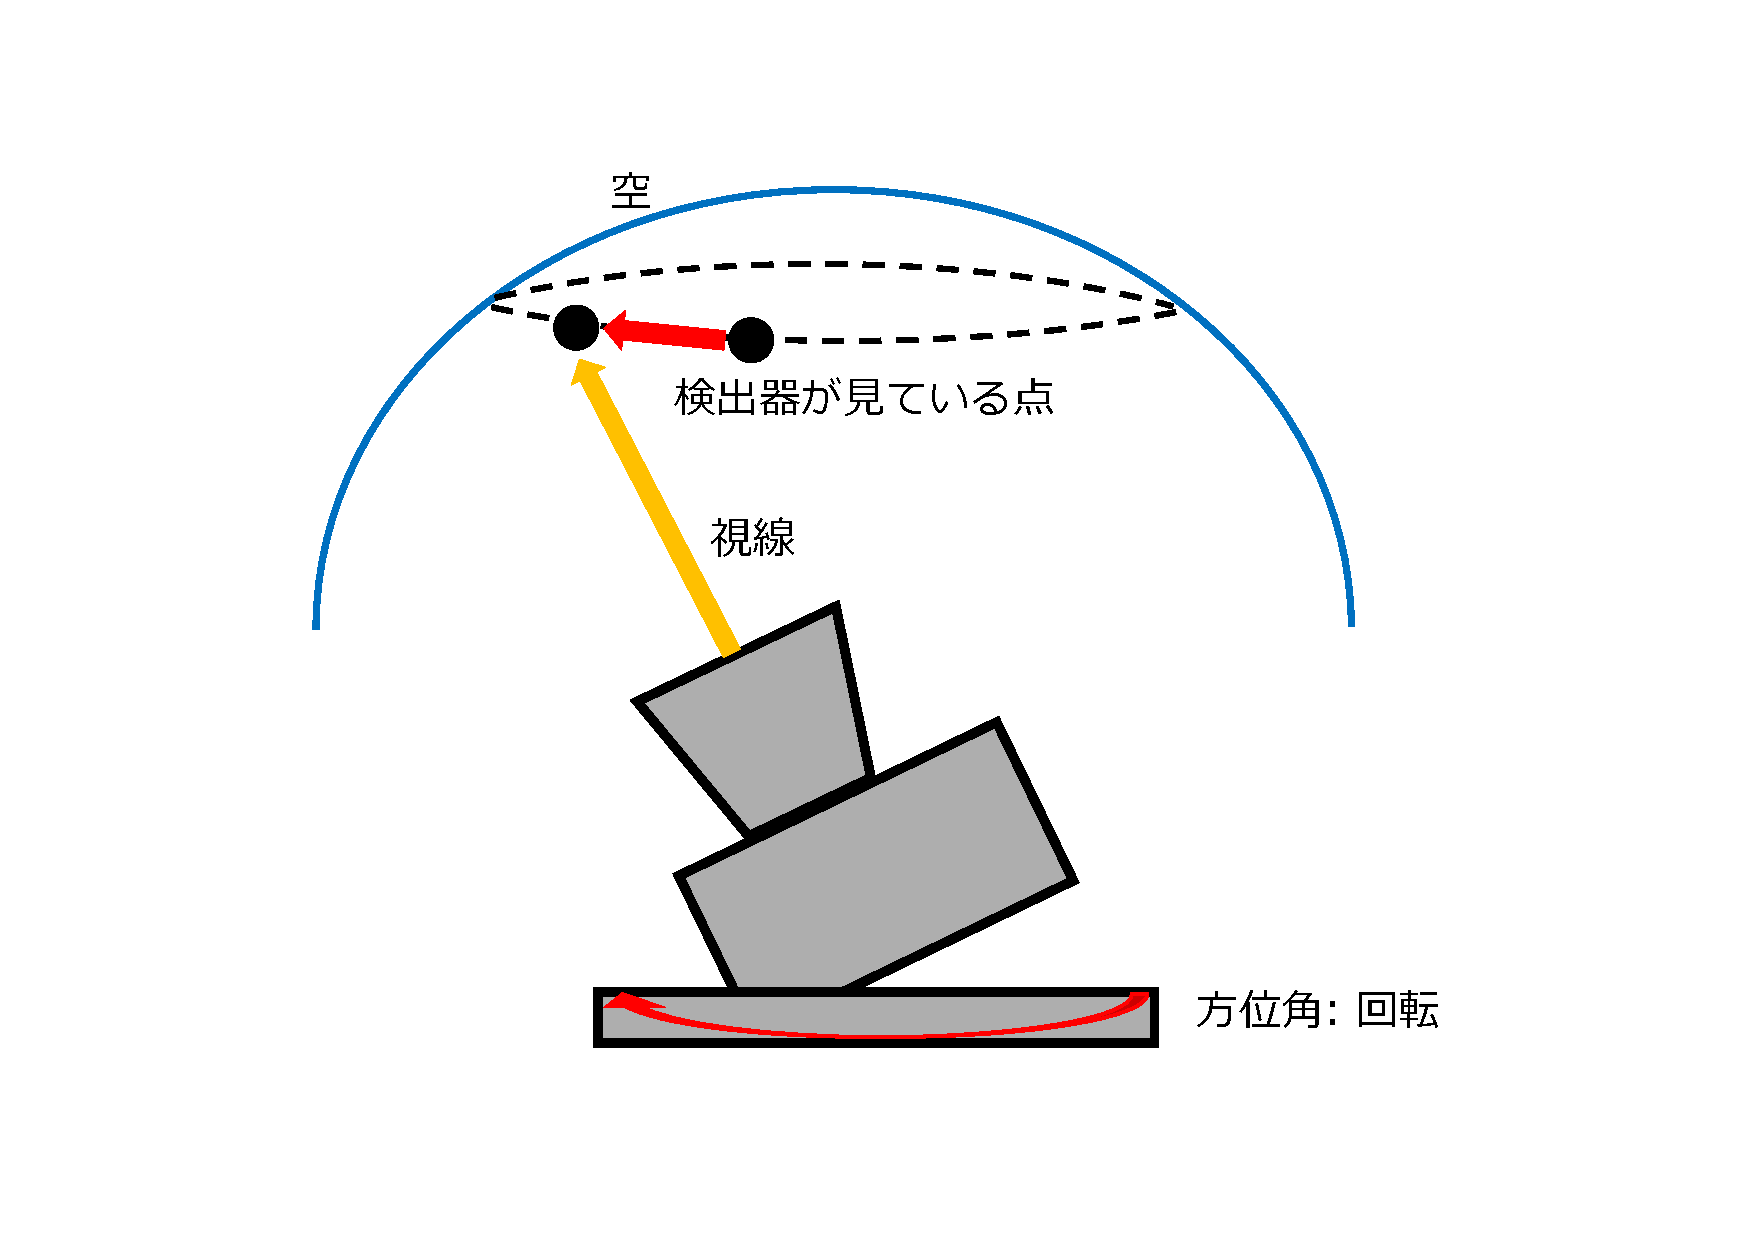
\includegraphics[width=0.6\columnwidth]{5_alignment/figs/scan_image.pdf}
  \caption{検出器が空の領域をスキャンする概要図。ある仰角を高速回転しながらスキャンする。}
  \label{scan_image}
\end{figure}
検出器で観測する信号は大きく(CMB + ノイズ)に分けられる。さらにノイズの中でも寄与が大きい成分に大気放射に由来するノイズがある。このノイズは刻一刻と変動する上に空の領域によっても異なっているため、高速回転によるスキャンで異なる検出器が同じ空の領域をスキャンすることで抑制できる。具体的には、異なる偏光方向に感度のある検出器が同じ仰角の空をスキャンする時、もう一方の検出器は片方の検出器が観測した空の領域をわずかな時間差で観測することができる。つまり、スキャンの間に大気の情報は変動せず観測される大気由来のノイズも変動しないことになる。そのため、検出器間で信号の差分をとることで、大気ノイズは共通していると考えれば取り除くことができ、偏光成分のみを残すことができる。しかし、検出器の配置がずれていて検出器間でスキャンする空の領域が異なる場合、大気の情報も異なり、差分をとっても大気ノイズを取り除くことができない(図\ref{scan_axis})。
\begin{figure}[htbp]
  \centering
  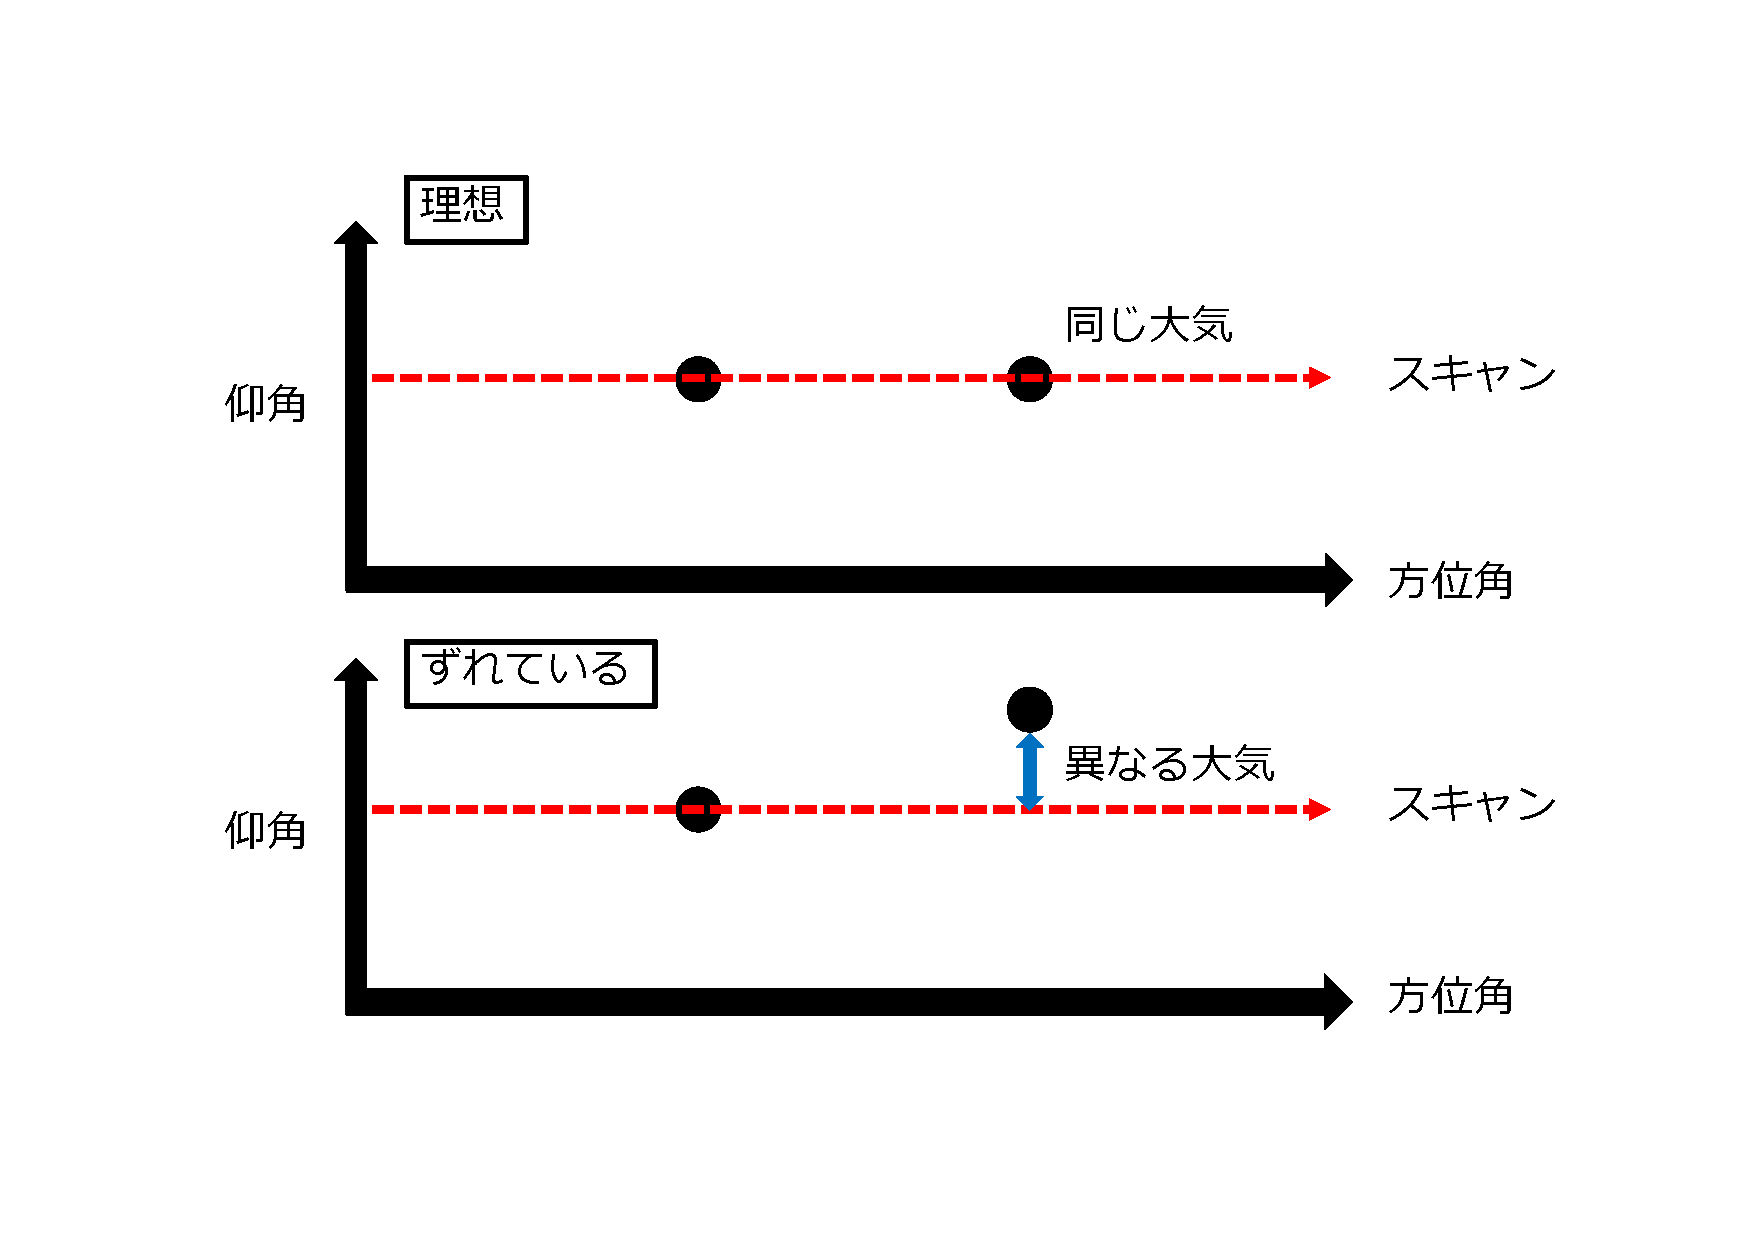
\includegraphics[width=0.7\columnwidth]{5_alignment/figs/scan_axis.pdf}
  \caption{空での理想的な検出器の配置とずれている場合の配置との比較。スキャン軸(方位角軸)に沿って検出器が並んでいないと観測する大気が検出器ごとに異なる。}
  \label{scan_axis}
\end{figure}

以上から空での理想的な検出器の配置は``複数の検出器がスキャン軸に沿って並んでいる''ことである。

しかし、観測データから理想的な検出器の配置からずれていることが示唆されていた。また、そのずれはスキャン軸に対して無視できないほどに有意な角度で傾いているものだと考えられていたが十分な検証と較正(実際に何度傾いているのか、傾きがあることでどれ程大気ノイズの影響が残ってしまうのか、など)がされていなかった。検出器アライメントの問題を改善し、GroundBIRDが持つ観測性能を最大限に引き出すことは質の良いデータを取得するためには不可欠である。

\subsection{要求される理想的なアライメント}

GroundBIRDにおける理想的な検出器の配置について詳細を見ていく。焦点面検出器は図\ref{full_array_picture}のように7つの検出器アレイが平面的に取り付けられているが、この検出器が観測する領域は平面のまま空に射影される訳ではない。観測する空の点は天球面上に張り付いた点と考えられるため、球面として射影される。焦点面検出器が平面を見るときと空を見る時での理想的な配置の違いを図\ref{distortion_pos}に示す。実際には球面から来る歪みの影響を受けた配置として空を観測することになり、望遠鏡の視線中心(\SI{220}{GHz}アレイ)ではほぼ平面だが、中心から離れた検出器は歪みの影響が出る。歪みを考慮した上で複数の検出器をスキャン軸に沿って並べることは焦点面の設計上難しい。また、高周波になるほど大気放射の寄与が大きくなる\cite{atmos_radiation}ことから、本論文では歪みの影響が少なく、大気放射の寄与も大きい中心の\SI{220}{GHz}アレイに対して配置がスキャン軸に沿って並んでいることを理想的なアライメントとする。
\begin{figure}[htbp]
  \centering
  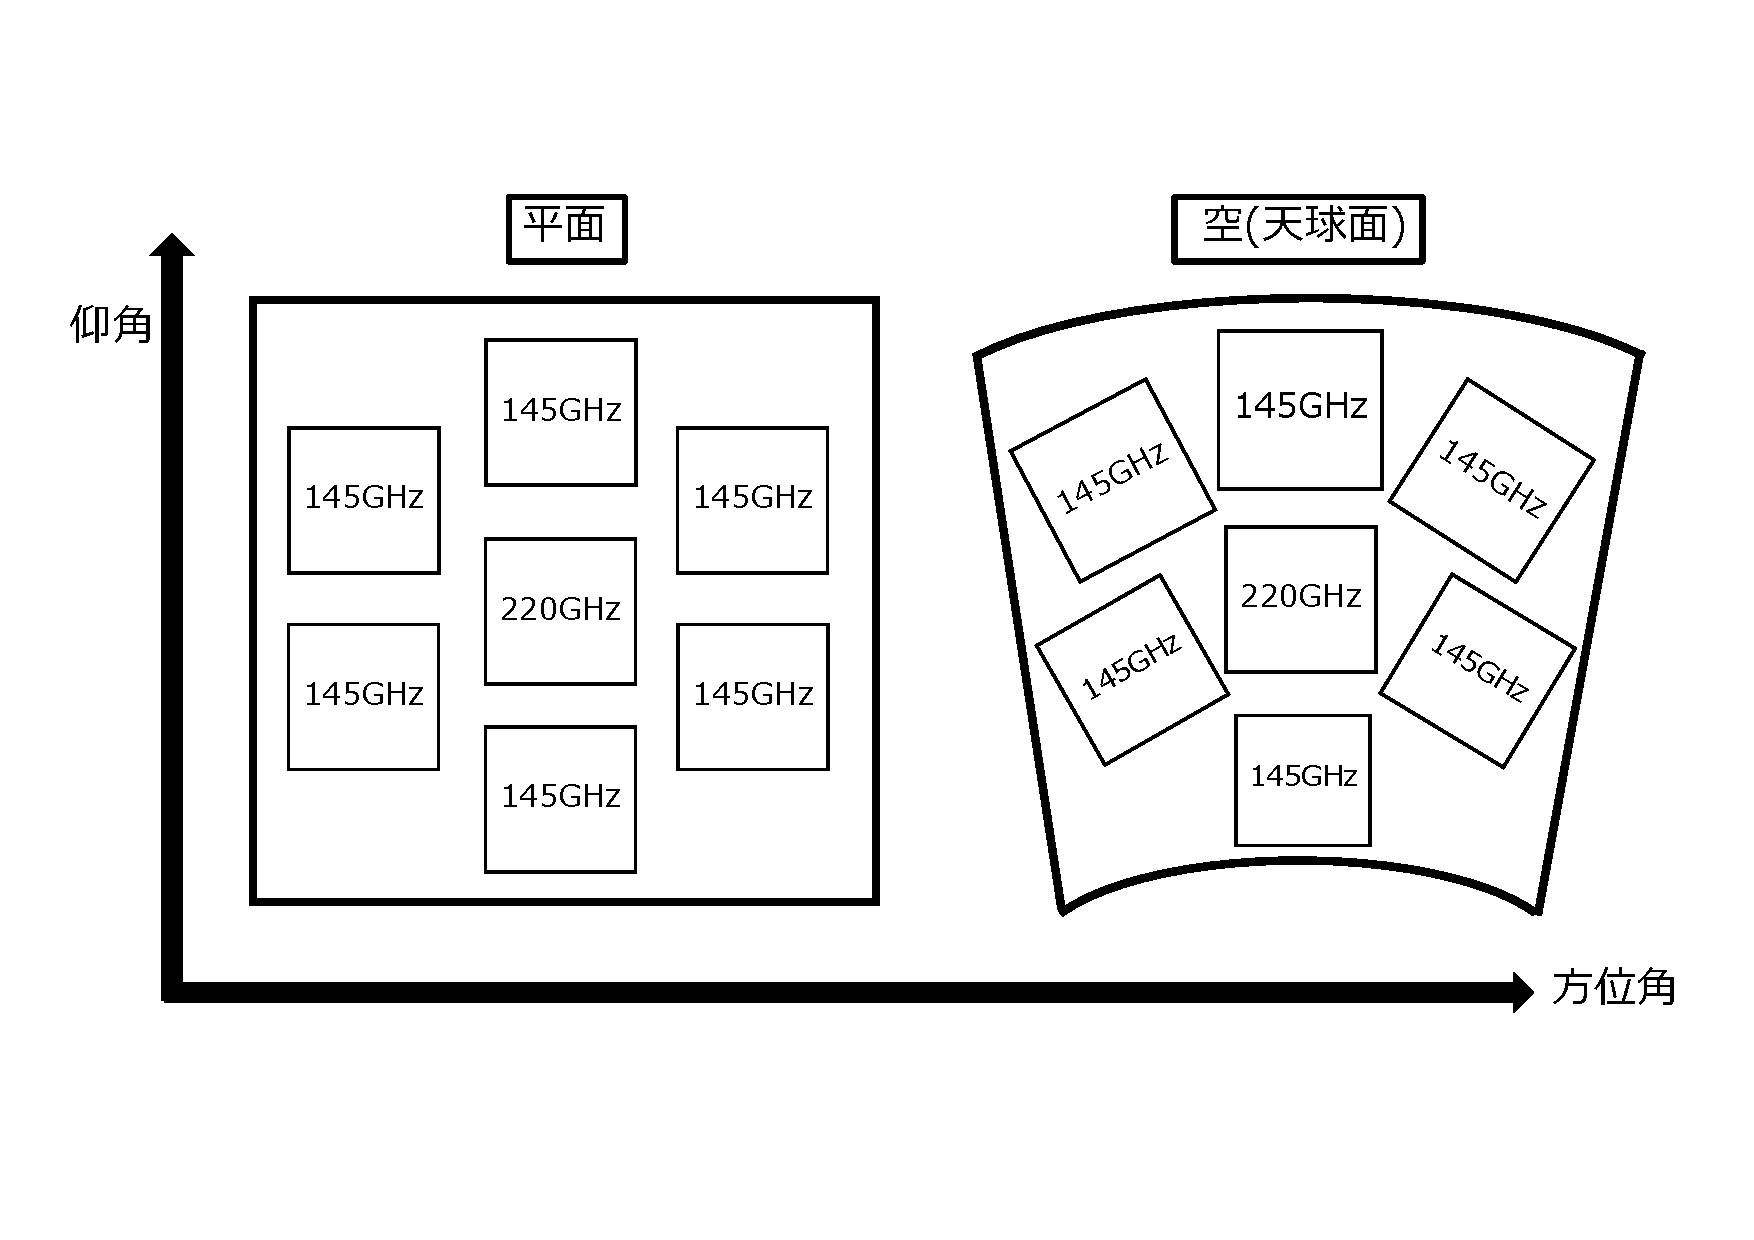
\includegraphics[width=0.8\columnwidth]{5_alignment/figs/distortion_pos2.pdf}
  \caption{平面と空(天球面)での理想的な検出器配置の違い。}
  \label{distortion_pos}
\end{figure}
\subsection{視線軸方向まわりの回転による較正}

スキャン軸に対して傾いた焦点面検出器を理想とする配置にするためには、検出器の視線を回転させてスキャン軸に並べれば良いことになる。また、焦点面検出器は望遠鏡内部で固定されているため望遠鏡全体の視線を回転することに対応する。つまり、望遠鏡のビーム中心を望遠鏡の視線方向とし、視線方向軸周りに適当な角度回転させることで各検出器の視線を回転させる(図\ref{boresight_axis})。
\begin{figure}[htbp]
  \centering
  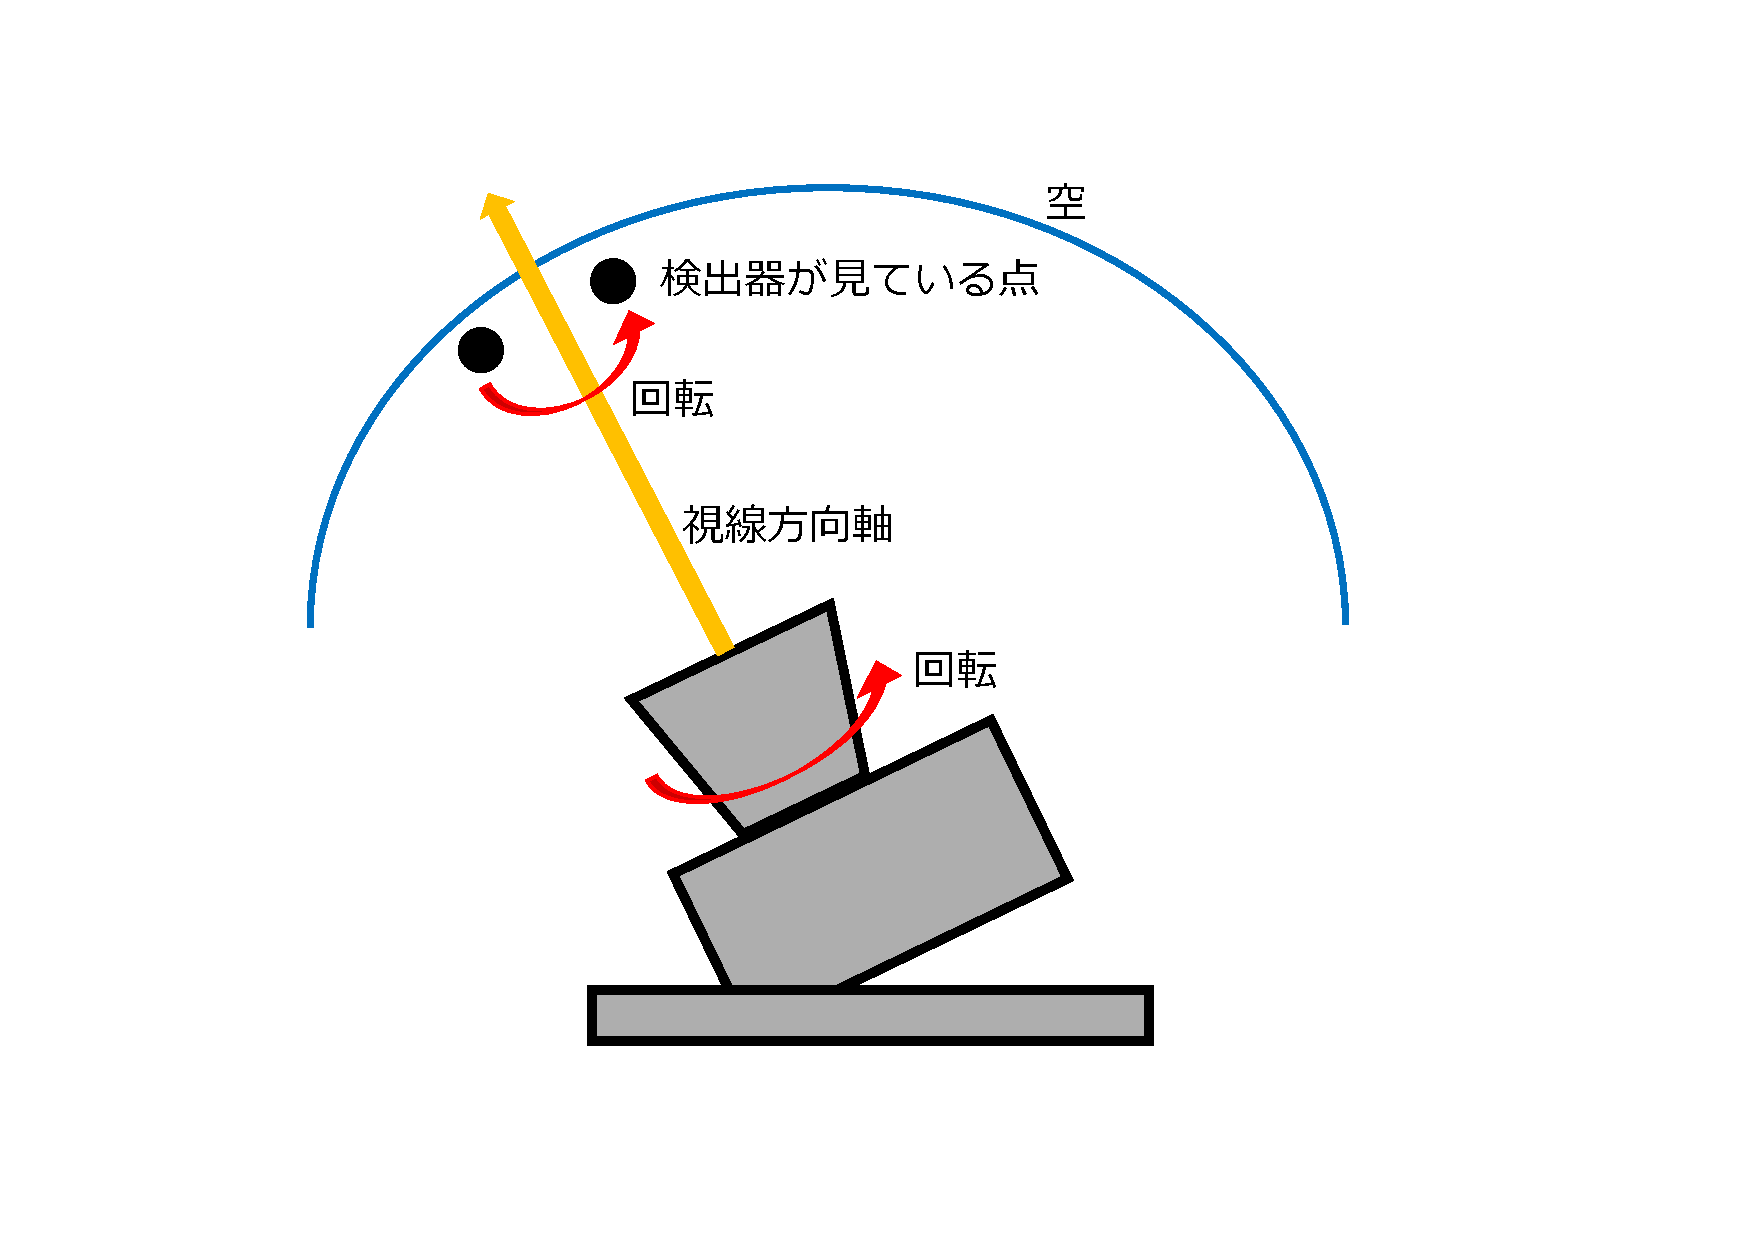
\includegraphics[width=0.8\columnwidth]{5_alignment/figs/boresight_axis.pdf}
  \caption{望遠鏡の視線方向軸と軸周りの回転。検出器の見ている点(視線)も回転する。}
  \label{boresight_axis}
\end{figure}
%検出器の配置がビームの中心に対して傾いている場合、視線方向軸の周りに望遠鏡を適当な角度回転させることで配置をスキャン軸に沿って並ばせることが可能になる。

そのため、理想的なアライメントにするための回転角を見積もる必要がある。回転角を求めるには各検出器の見ている点を知る必要があり、天体の観測データを解析することで算出できる(天体の運動が分かっているので検出器データと角度データから各検出器の視線情報を求められる)。

\section{月を用いた回転角の算出}

\subsection{月を用いた理由}

GroundBIRDで観測できる天体として月や惑星(木星、金星)が挙げられる。しかし、月と惑星ではデータの性質は大きく異なり、それぞれ観測上の長所と短所が存在する。月データと惑星データの特徴を表\ref{moon_vs_planet}に示す。
\begin{table}[htbp]
  \centering
  \caption{月データと惑星データの比較\cite{sueno_doctor}}
  \vspace{3mm}
  \begin{tabular}{ccc} \hline
    & 月 & 惑星 \\ \hline
    長所 &
    \begin{tabular}{c}
    S/N比が高い \\ (1度の観測で十分な信号を得られる)
    \end{tabular} &
    \begin{tabular}{c}
    点源として扱える \\ (視野角がビーム幅に比べて十分小さい)
    \end{tabular} \\ \hline
    短所 &
    \begin{tabular}{c}
    点源として扱えない \\ (輝度温度の非一様性が生じる)
    \end{tabular} &
    \begin{tabular}{c}
    S/N比が小さい \\ (データを蓄積しないとノイズに埋もれる)
    \end{tabular} \\ \hline
  \end{tabular}
  \label{moon_vs_planet}
\end{table}
検出器の視線情報を得るには点源として扱え、正確に点として求められる惑星が適しているが、\ref{jupiter_ana}で見るように点源で最も明るい木星の観測データでもノイズの影響をかなり受けてしまう。そのため、データを蓄積するか、PWVや湿度が十分低く観測条件が整った観測データを使用する必要がある。一方、月は高いS/N比により1度の観測データで十分な信号を得られ、データを蓄積することによるノイズが加わることなく解析ができる。点源として扱えないことによる誤差はあるものの、高いS/N比がそれをカバーできると考えたため、月のデータを選択した。

\subsection{位相としての検出器TOD}
GroundBIRDにおける観測データは\ref{MKID}で述べた超伝導検出器MKIDの共振状態の変化を入射信号の大きさとして\SI{1}{kSPS}で取得するTODのことである。共振状態の変化とはすなわち共振周波数の変化であるが、これを読み出しRF信号の透過率の変化として測定する。透過率は散乱行列要素の$S_{21}$で表す。MKIDの$S_{21}$は共振の鋭さを表す$Q_{r}$, $Q_{c}$を用いて
\begin{equation}
  |S_{21}-x_{c}| = \frac{Q_{r}}{2Q_{c}} \bigl(x_{c} = 1-\frac{Q_{r}}{2Q_{c}}\bigr)
\end{equation}
で得られ\cite{muto}、$S_{21}$の軌跡が円状になることが分かる。この円は``共振円''と呼ばれる。共振円と$S_{21}$の例を図\ref{res_circ}に示す。
\begin{figure}[htbp]
  \centering
  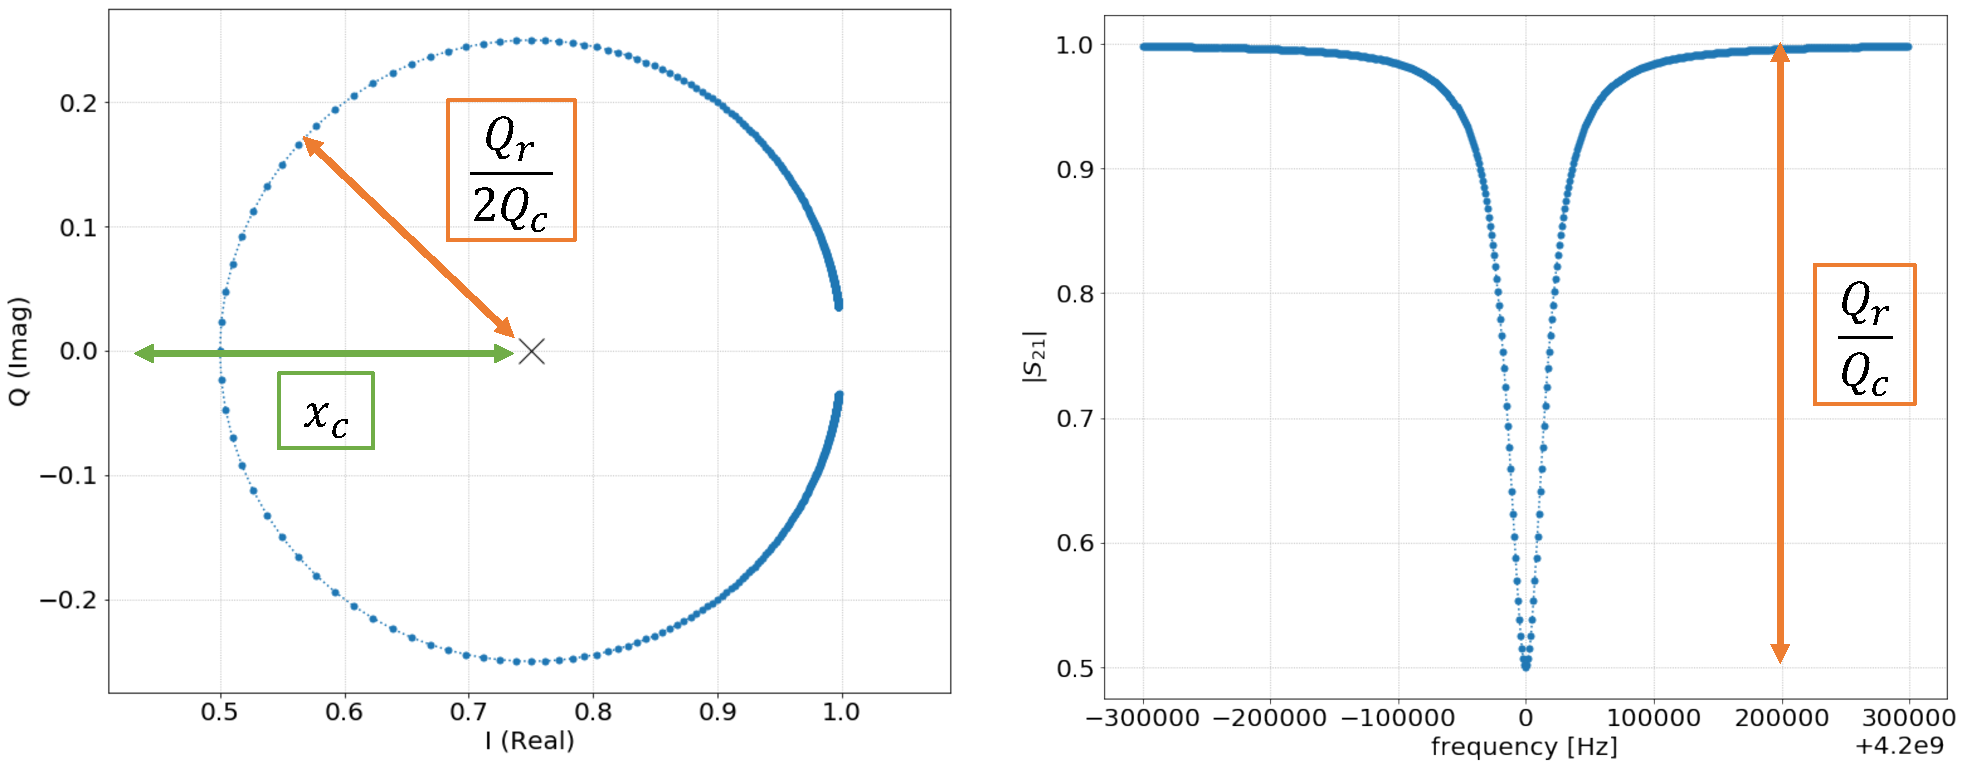
\includegraphics[width=1.0\columnwidth]{5_alignment/figs/iq_amp.pdf}
  \caption{共振円と共振周波数付近での透過率。\cite{sueno_master}より引用。}
  \label{res_circ}
\end{figure}
共振周波数の周りで透過率が鋭いピークを持つことが分かる。共振円を動く$S_{21}$の振幅$A$と位相$\theta$を
\begin{equation}
  A = \frac{|S_{21}|- x_{c}}{1-x_{c}}
\end{equation}
\begin{equation}
  \tan\theta = \frac{\mathrm{Im}(S_{21})}{x_{c}- \mathrm{Re}(S_{21})}
\end{equation}
と定義する。これらの値は共振周波数の変化に対して敏感であるため、振幅の変化($\delta A$)と位相の変化($\delta\theta$)によって入射信号の大きさを読み出せる。入射信号によって振幅と位相が変化する例を図\ref{amp_and_phase}に示す。
\begin{figure}[htbp]
  \centering
  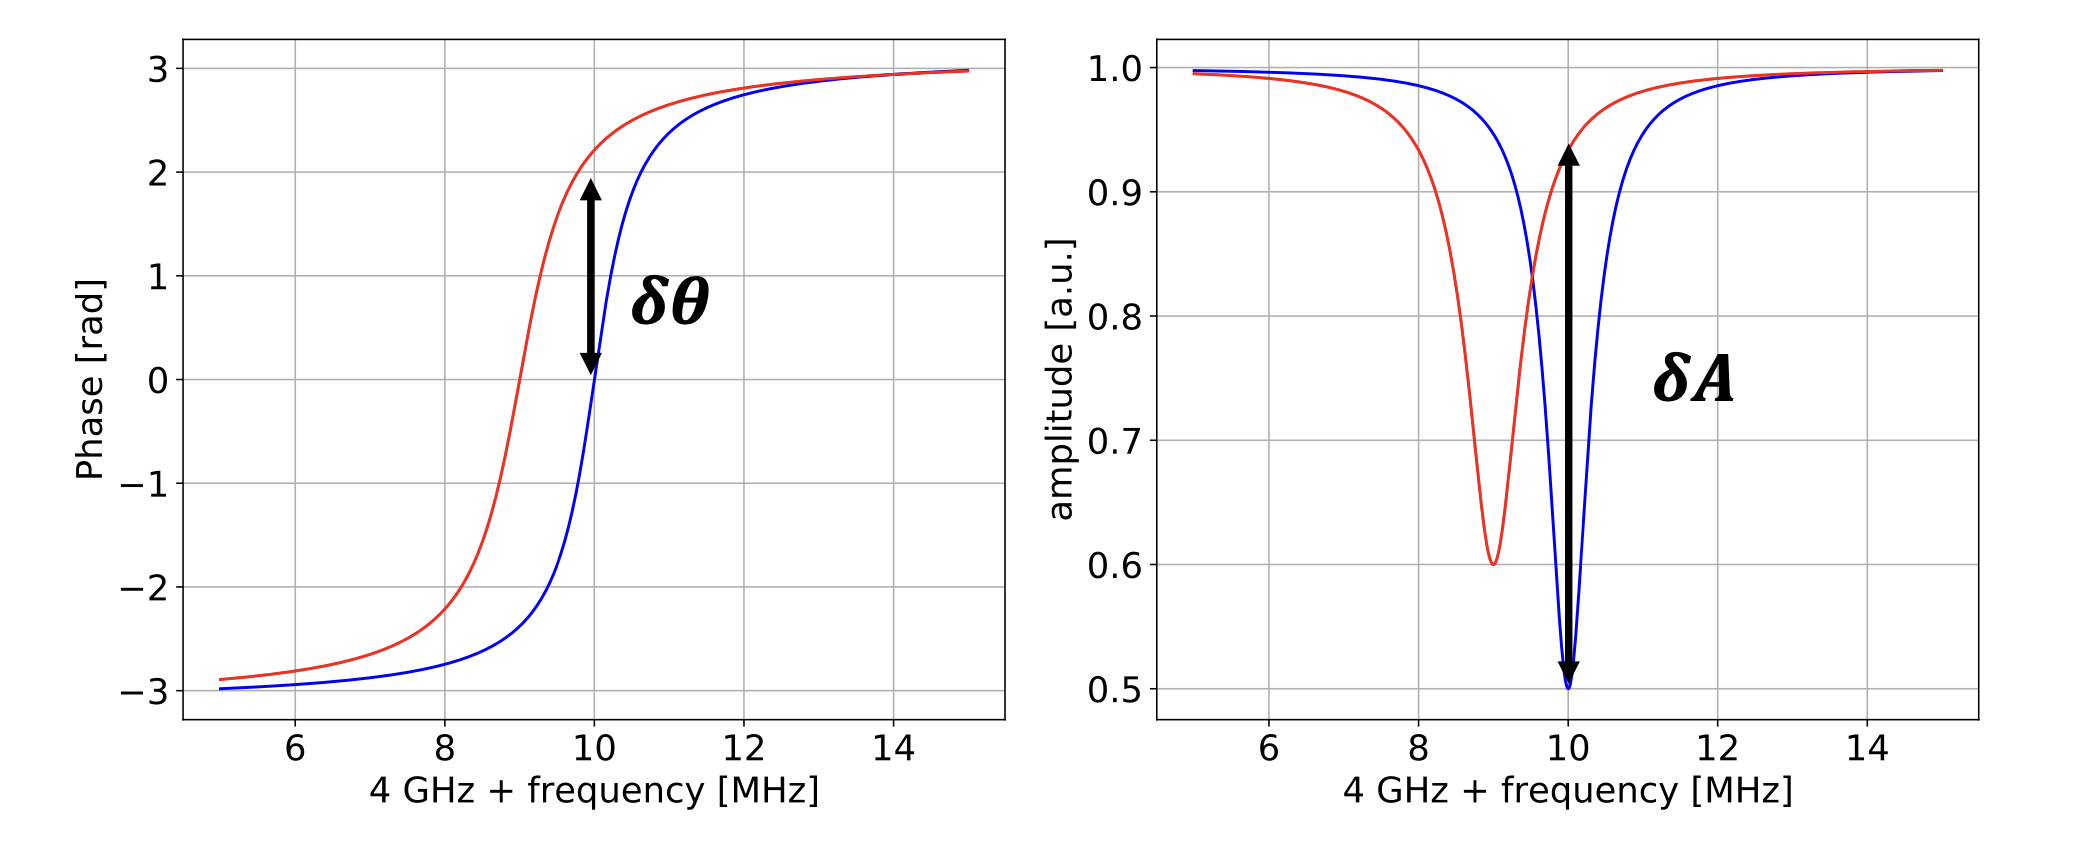
\includegraphics[width=1.0\columnwidth]{5_alignment/figs/amp_and_phase.png}
  \caption{共振周波数付近での$S_{21}$の振幅と位相の変化。\cite{sueno_doctor}より引用。}
  \label{amp_and_phase}
\end{figure}

実際のTOD取得時には図\ref{amp_and_phase}のように各MKIDで固定した共振周波数で測定を行う。そのため、TOD取得前に各MKIDの共振周波数を知る必要がある。また、共振周波数は観測条件によって変動するため、一定の値をとらない。そのため、1観測を1時間で区切っており、1観測ごとにTOD取得前に共振周波数を求めている(その間も望遠鏡は連続的に稼働している)。共振周波数を知るために
\begin{enumerate}
  \item 周波数スイープ
  \item フィッティング
\end{enumerate}
の手順で測定をする。周波数スイープとは、読み出し用のRF信号の周波数を少しずつ変えながら測定をする手法である。測定量はRFの透過率で、スイープで測定されたデータを透過率の関数でフィットすることで共振周波数を求める。フィット関数は$S_{21}$に補正項を入れたもので
\begin{equation}
  T_{21}(f) = a_{0}~\mathrm{exp}(-2\pi if\tau_{0})\biggl(1-\frac{Q_{r}/Q_{c}e^{i\phi}}{1+2iQ_{r}(f-f_{r})/f_{r}}\biggr)
\end{equation}
で表される\cite{sueno_master}。ここで、$a_{0}$, $\tau_{0}$は読み出し回路による振幅の減衰と位相のずれを表す。$e^{i\phi}$はCカップリングでのインピーダンスを補正する項である。このフィットで共振周波数$f_{r}$と共振の鋭さを表す$Q_{r}$, $Q_{c}$を得られる。得られた$f_{r}$にRF周波数を固定し、TODを取得する。TODでの測定量は$T_{21}$であり、補正項の効果を差し引くことで$S_{21}$としての振幅$A$と位相$\theta$を取得できる。
%\begin{equation}
  %|S_{21}-x_{c}| = \frac{Q_{r}}{2Q_{c}} \bigl(x_{c} = 1-\frac{Q_{r}}{2Q_{c}}\bigr)
%\end{equation}
%で得られ\cite{muto}、$S_{21}$の軌跡が円状になることが分かる。この円は``共振円''と呼ばれる。共振円と$S_{21}$の例を図\ref{res_circ}に示す。
%\begin{figure}[htbp]
  %\centering
  %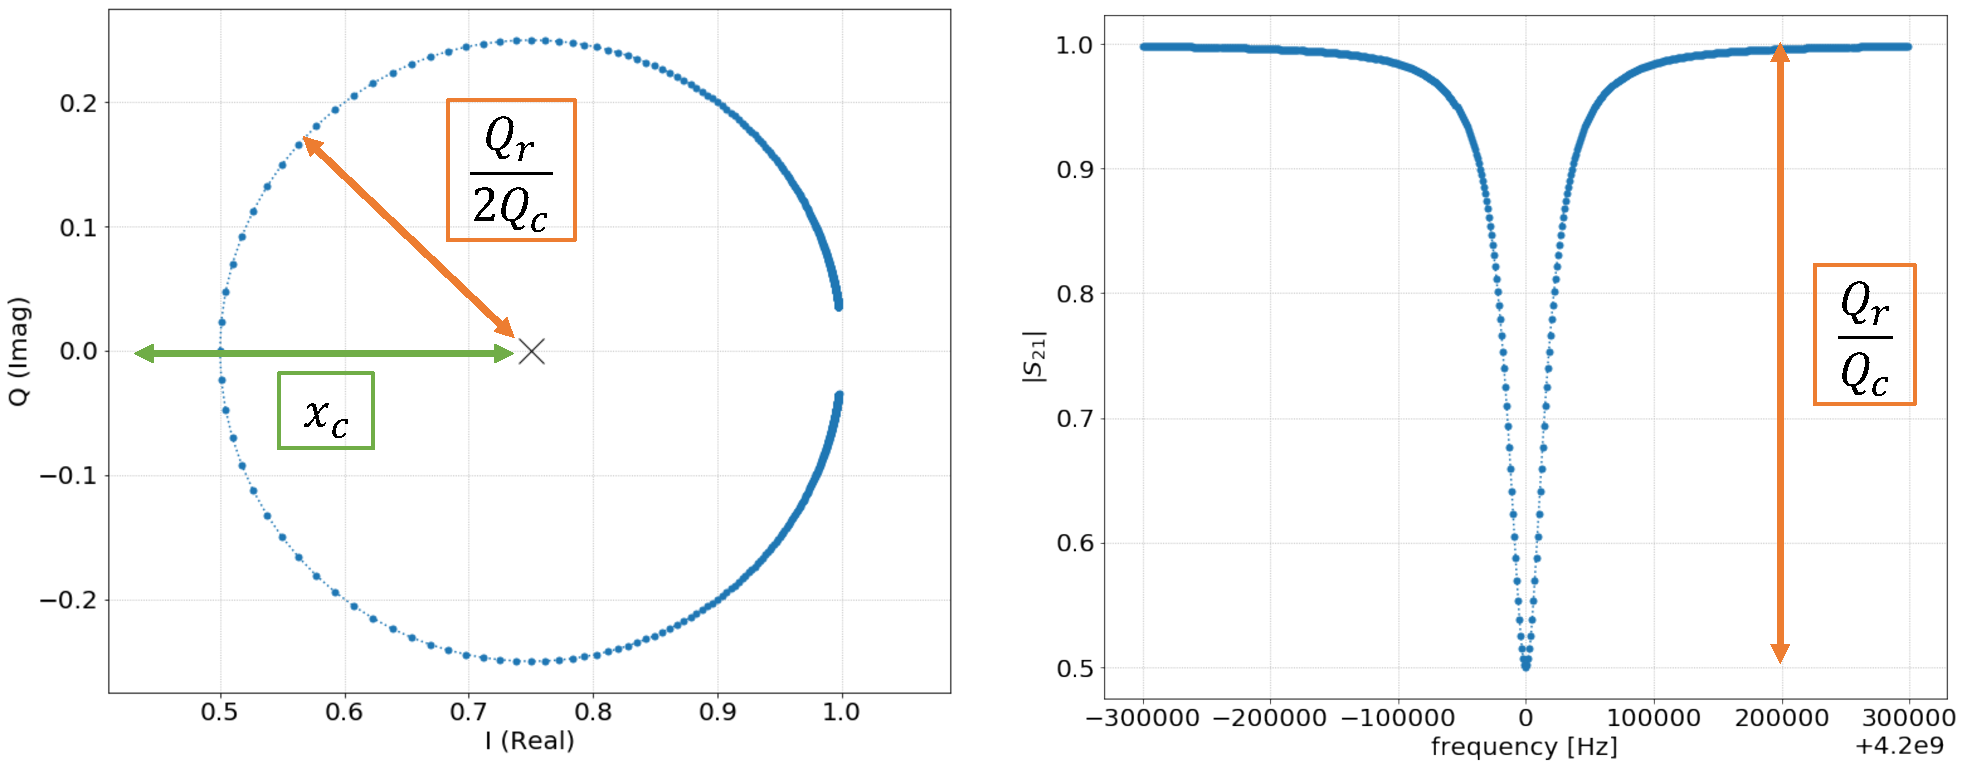
\includegraphics[width=0.9\columnwidth]{5_alignment/figs/iq_amp.pdf}
  %\caption{共振円と共振周波数付近での透過率。\cite{sueno_master}より引用。}
  %\label{res_circ}
%\end{figure}
%共振周波数の周りで透過率が鋭いピークを持つことが分かる。共振円を動く$S_{21}$の振幅$A$と位相$\theta$を
%\begin{equation}
  %A = \frac{|S_{21}|- x_{c}}{1-x_{c}}
%\end{equation}
%\begin{equation}
  %\tan\theta = \frac{\mathrm{Im}(S_{21})}{x_{c}- \mathrm{Re}(S_{21})}
%\end{equation}
%と定義する。これらの値は共振周波数の変化に対して敏感であるため、振幅の変化($\delta A$)と位相の変化($\delta\theta$)を測定することで入射信号の大きさを読み出せる。入射信号によって振幅と位相が変化する例を図\ref{amp_and_phase}に示す。
%\begin{figure}[htbp]
  %\centering
  %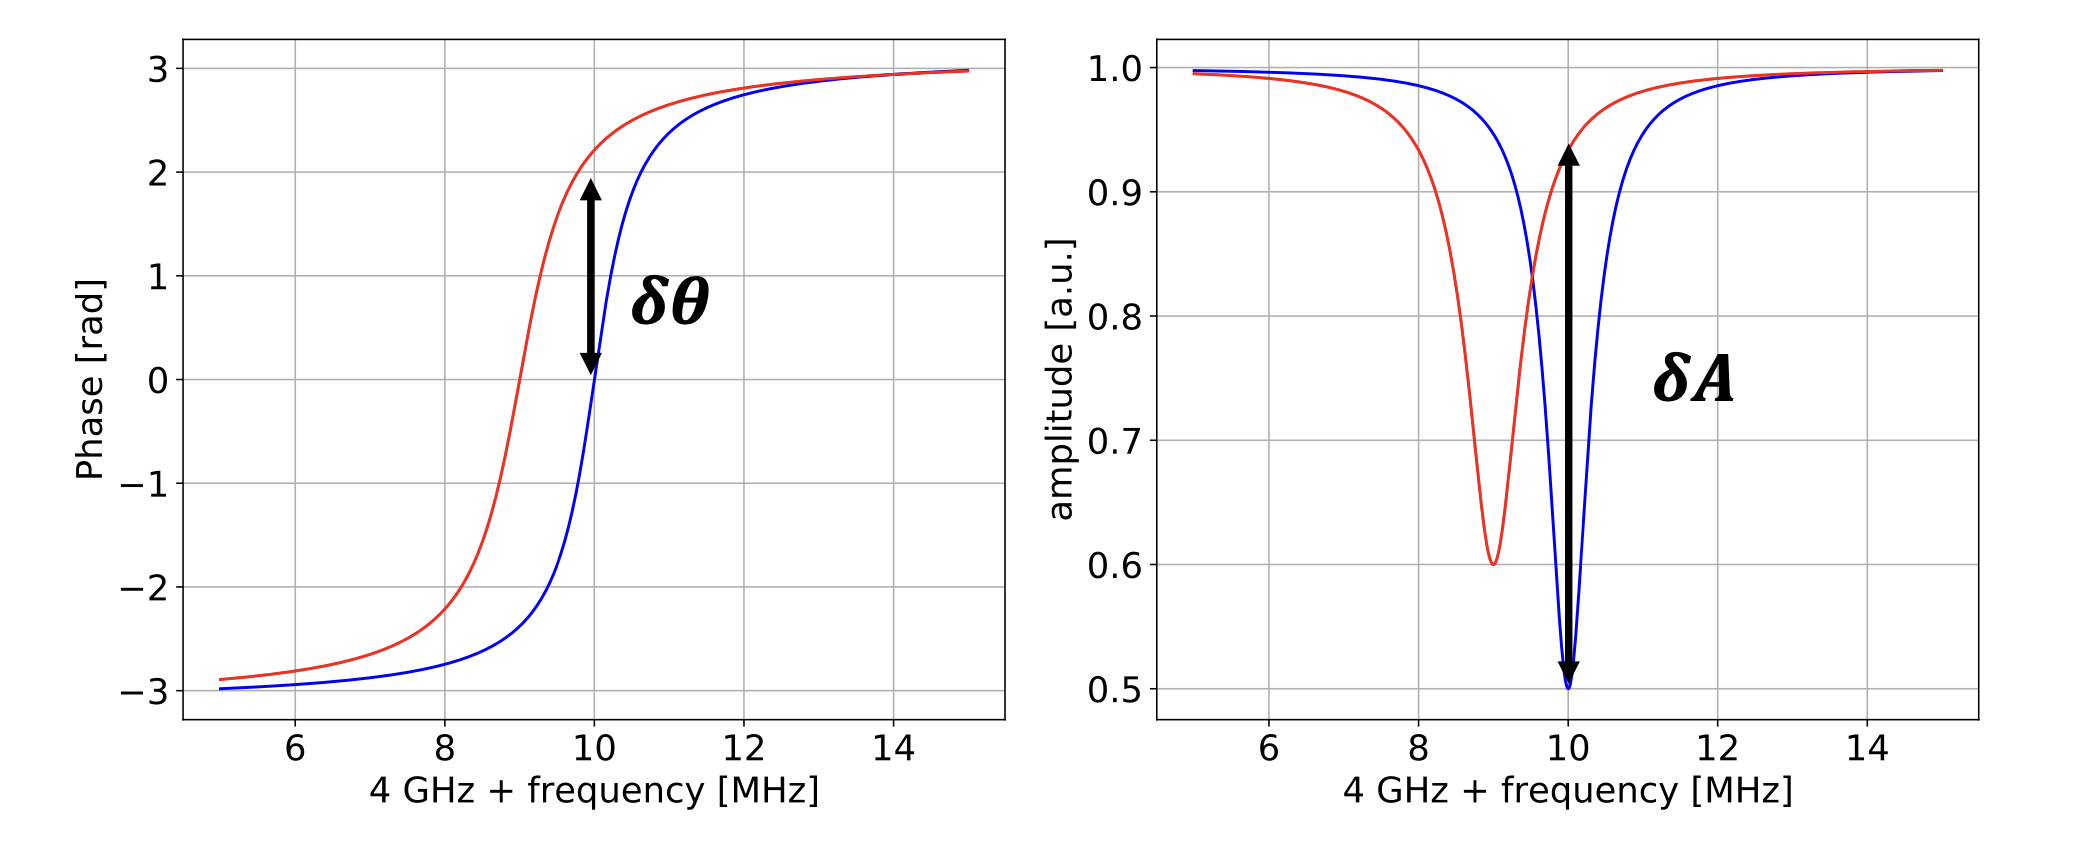
\includegraphics[width=1.0\columnwidth]{5_alignment/figs/amp_and_phase.png}
  %\caption{共振周波数付近での$S_{21}$の振幅と位相の変化。\cite{sueno_doctor}より引用。}
  %\label{amp_and_phase}
%\end{figure}
本論文ではより応答性の高い位相をTODとして使用する。また、非線形効果を補正したものを最終的に使用する位相TODとした。非線形効果の補正は位相の応答($\theta_{\mathrm{res}}$)に対して以下の式\cite{sueno_doctor}を用いた。
\begin{equation}
  \theta = 2\tan(\theta_{\mathrm{res}}/2)
\end{equation}
最終的に使用する位相TODの例(1観測)を図\ref{raw_phase}に示す。
\begin{figure}[htbp]
  \centering
  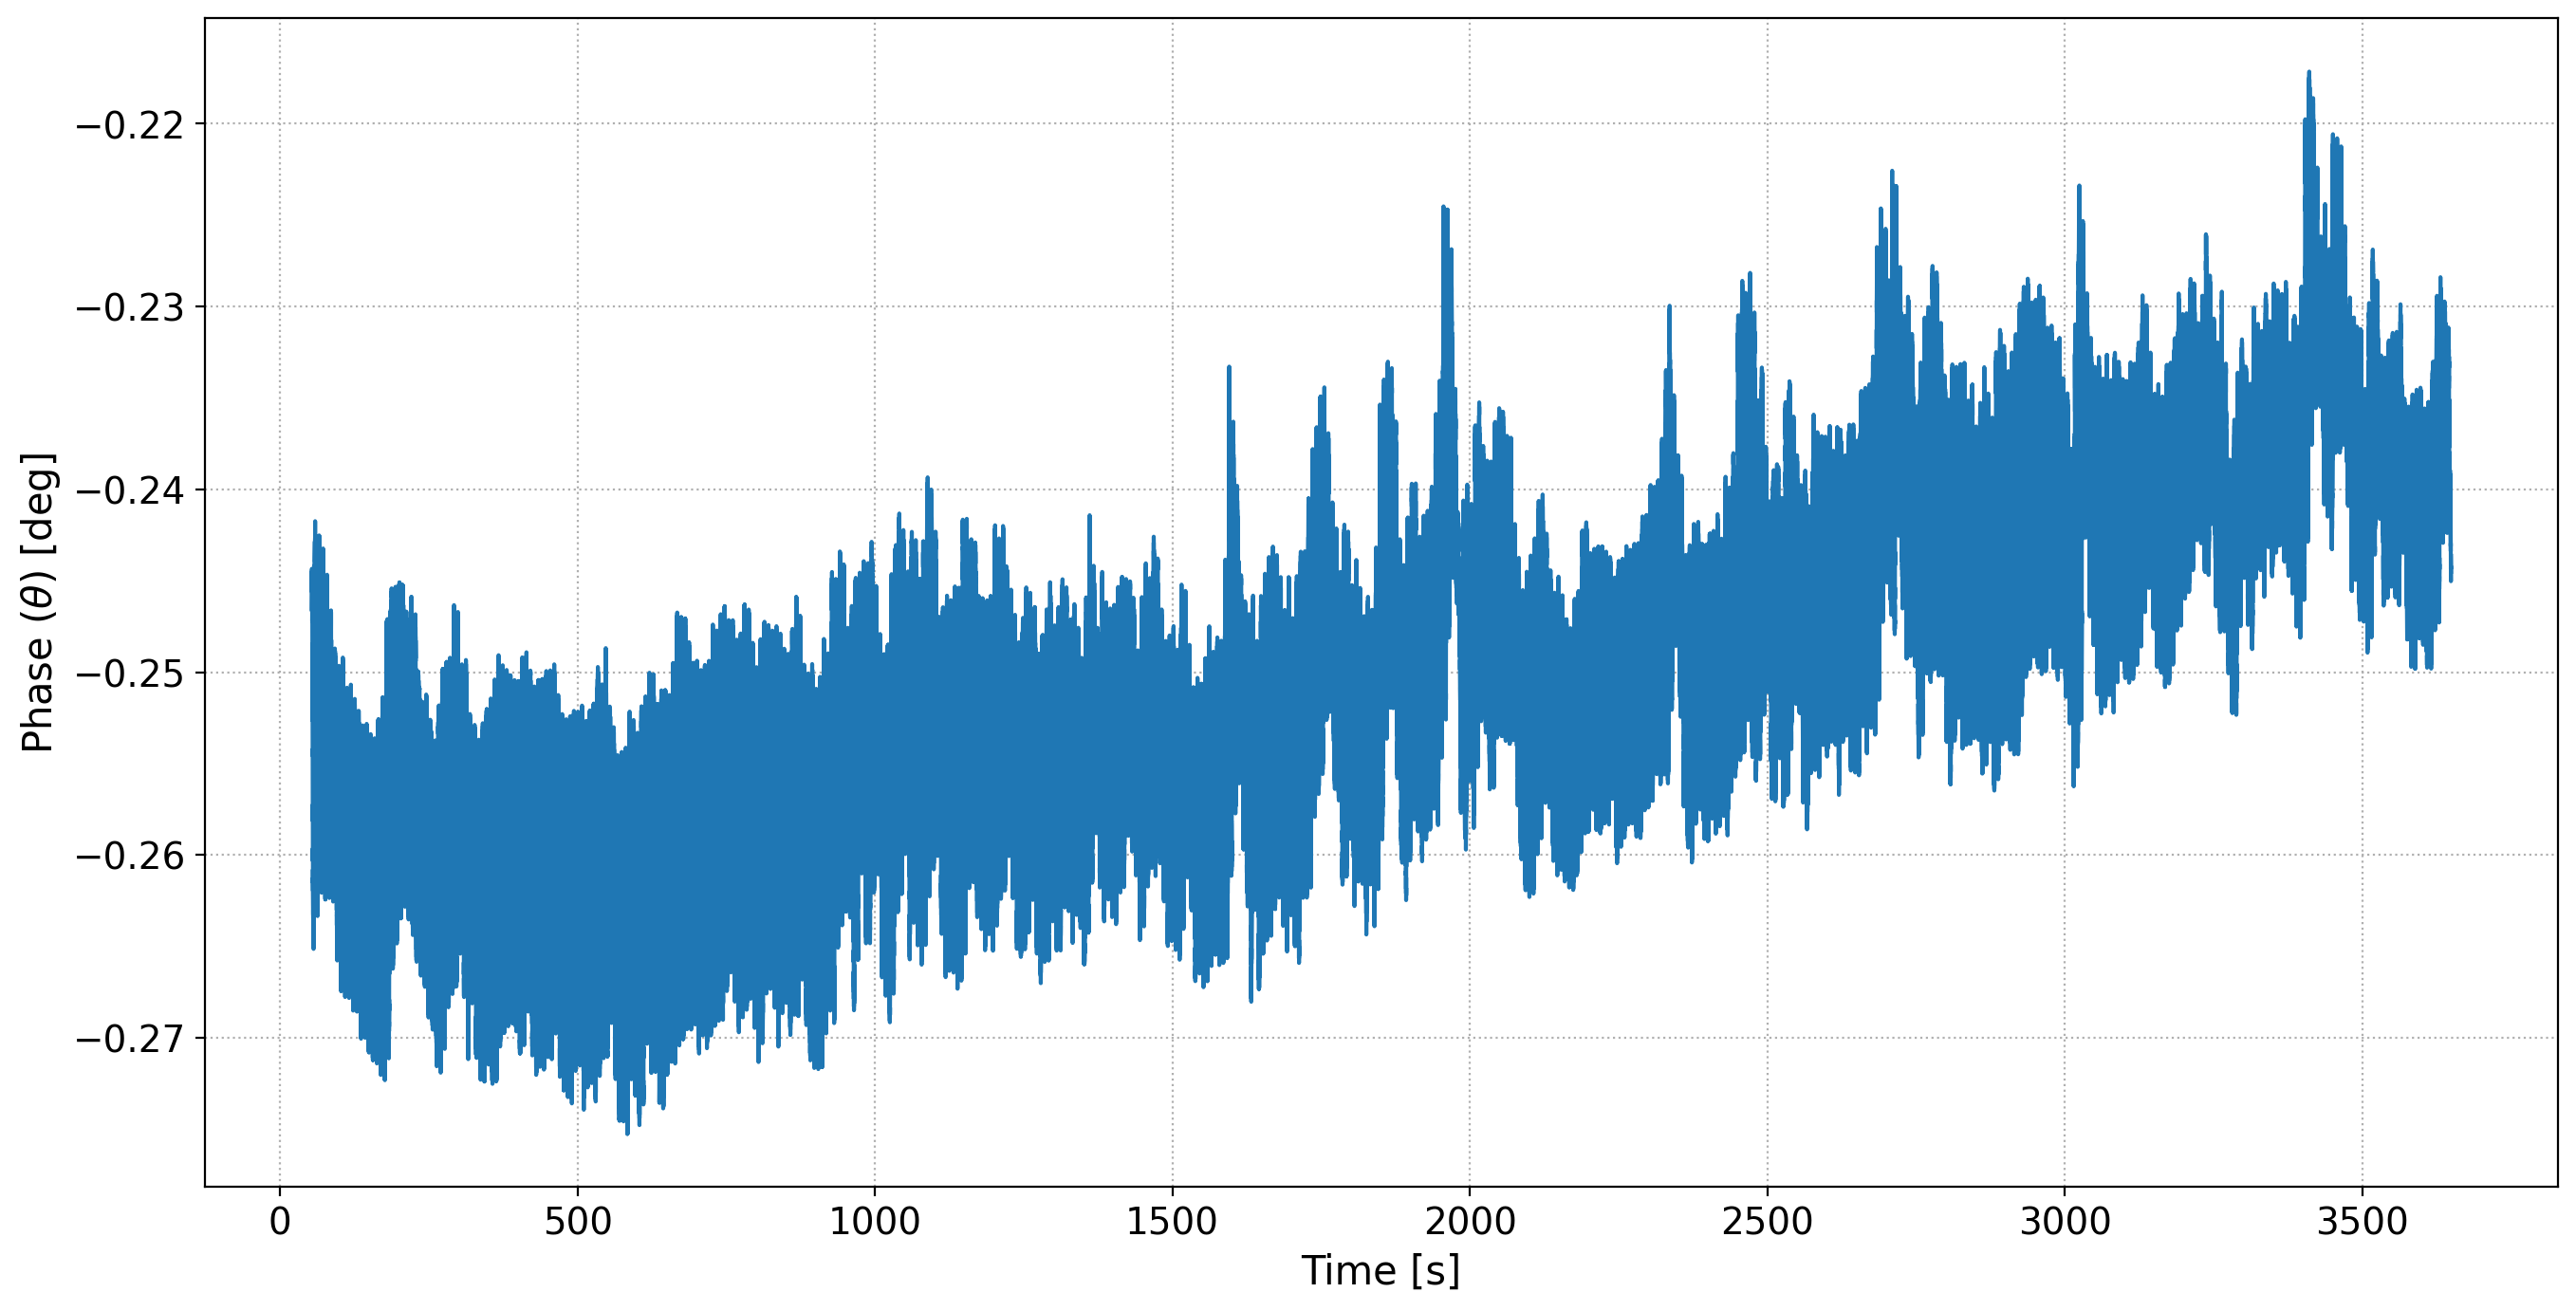
\includegraphics[width=0.9\columnwidth]{5_alignment/figs/raw_phase_deg.png}
  \caption{非線形効果を加えた位相TOD。本論文ではこのTODを用いる。}
  \label{raw_phase}
\end{figure}

\subsection{必要な回転角}
月の信号は大きく1観測のTODで鮮明なマップを得ることができる。月を観測した時(2023/12/02、1時間)の位相TODを図\ref{6550_kid0_phase}に示す。
\begin{figure}[htbp]
  \centering
  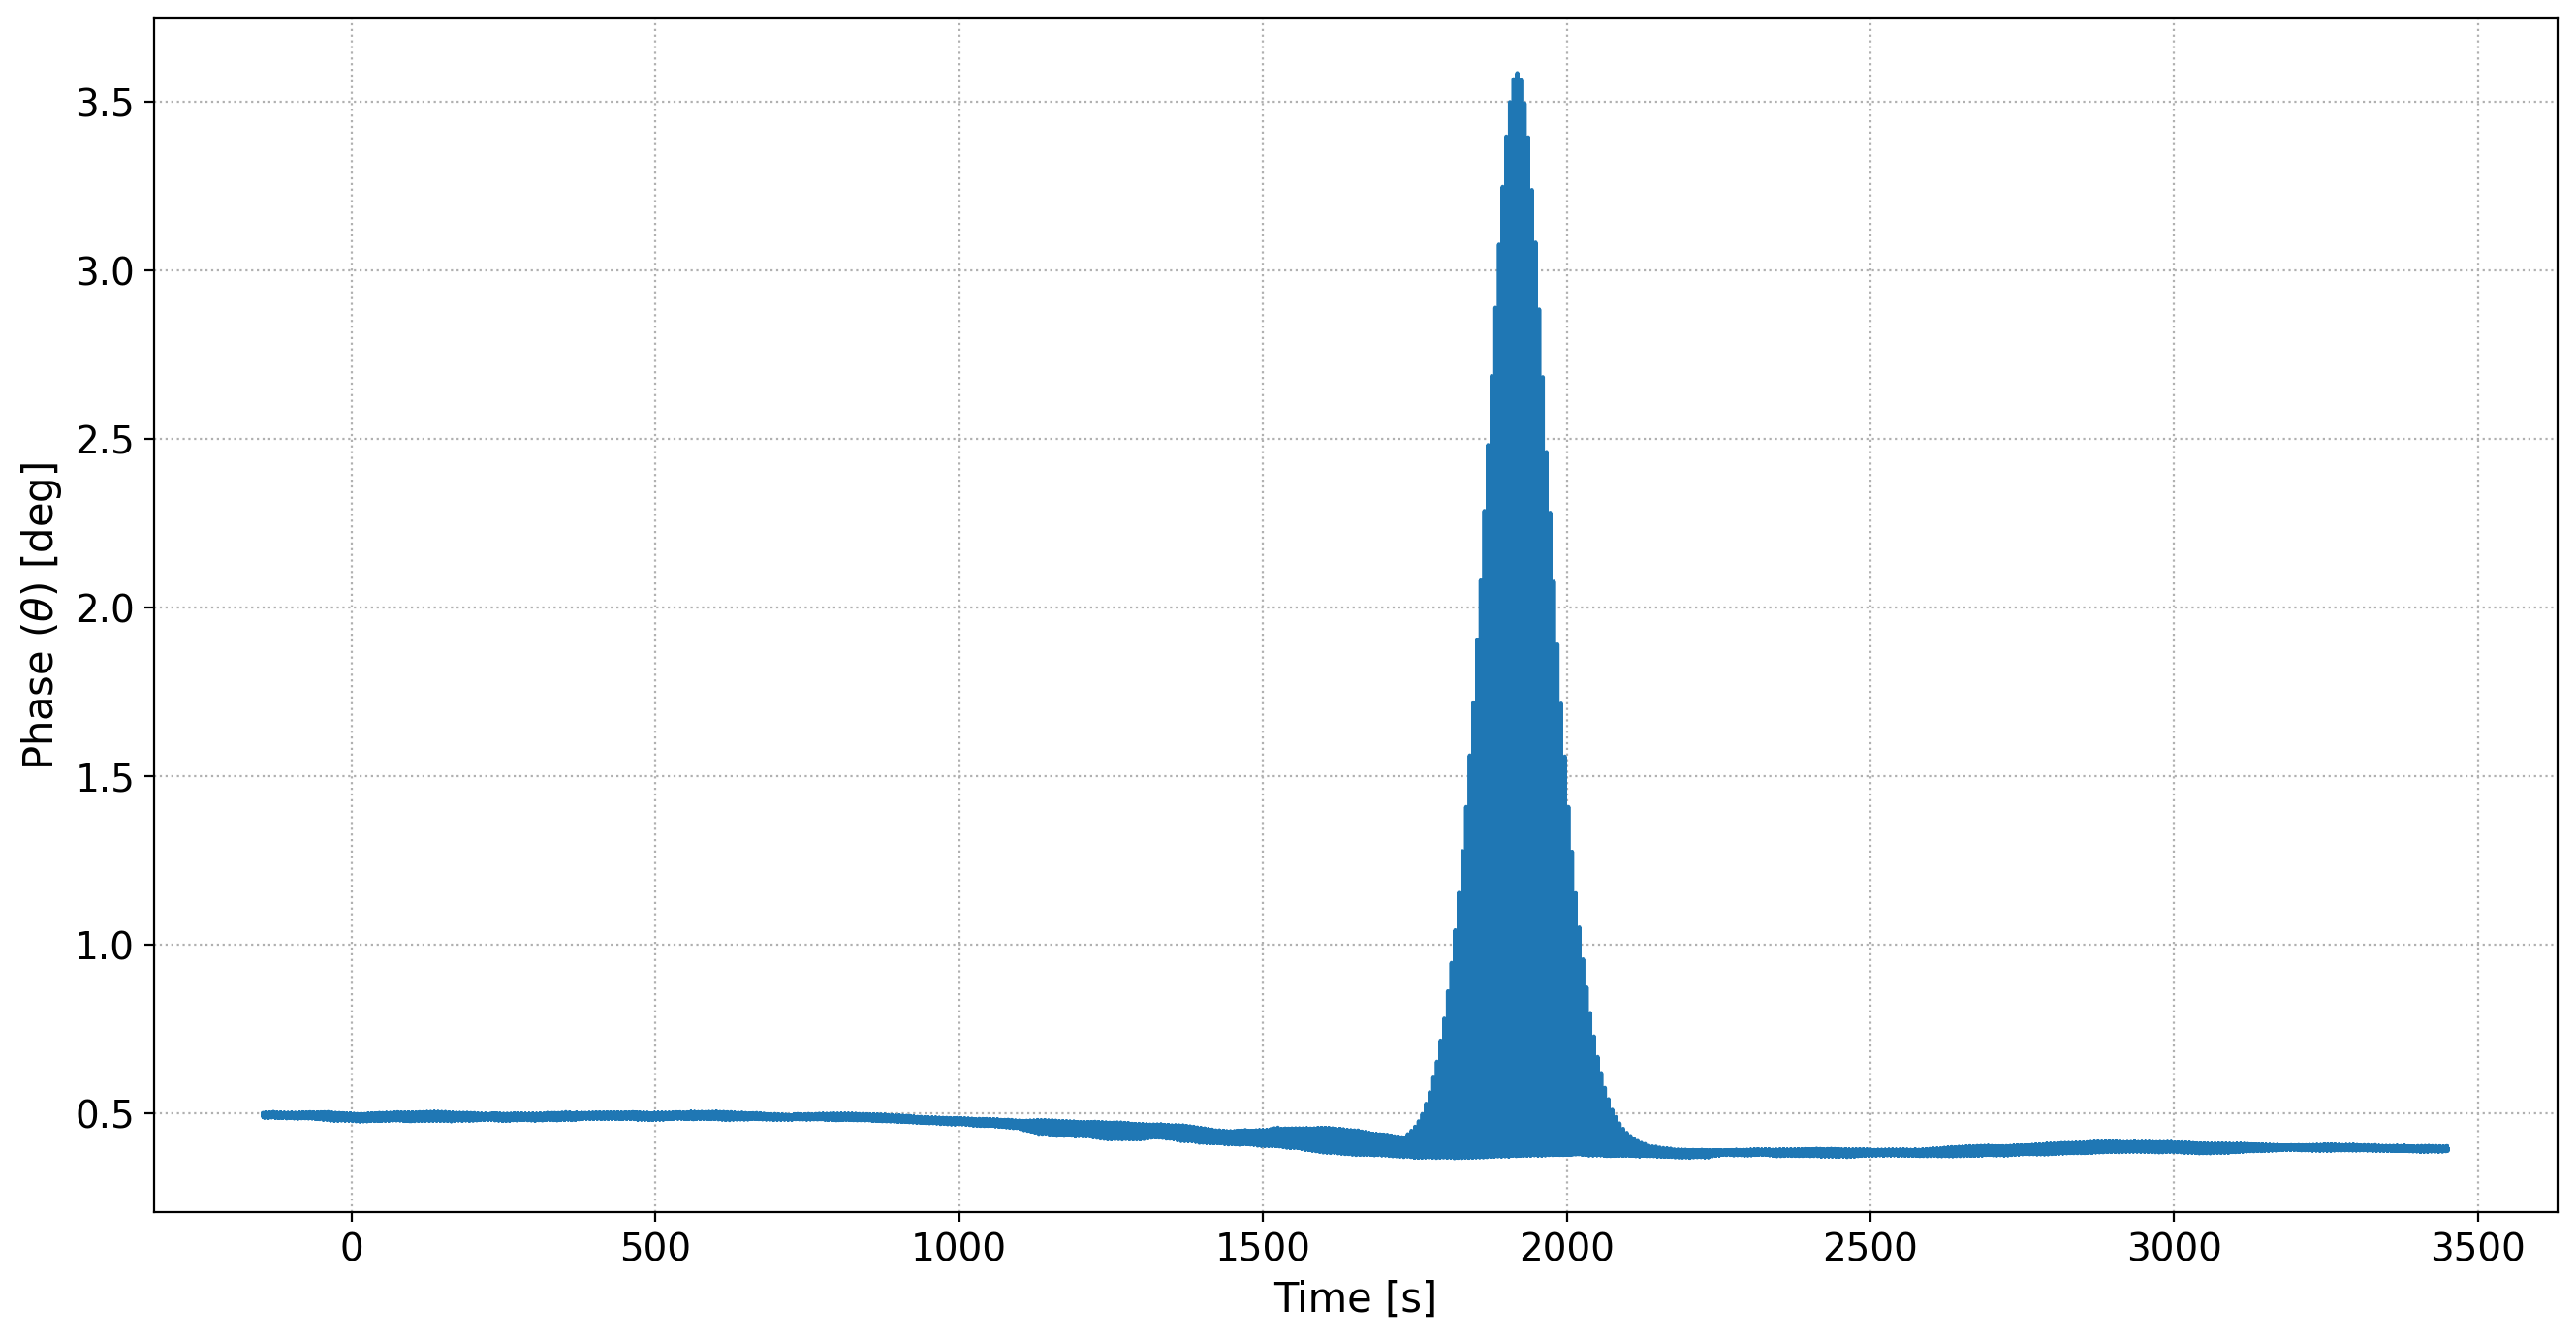
\includegraphics[width=0.85\columnwidth]{5_alignment/figs/6550_kid0_phase.png}
  \caption{月観測時のTOD。月の中心を観測した時にピークを取る。}
  \label{6550_kid0_phase}
\end{figure}
月は空を動いているが、望遠鏡が仰角を$\SI{70}{^{\circ}}$に固定してスキャンする間に月が望遠鏡の視野を通り過ぎる時に観測できる。つまり、1日の間に月が``昇る''時と``沈む''時とで2回の観測ができる。また、月の視野角は$\SI{30}{'}$であり点源とはみなせない。そのため図\ref{6550_kid0_phase}にあるように、月の端を観測する時と中心を観測する時では入射する信号の大きさが異なり、中心で最も強い信号を観測する。

月の運動はよく知られており、Pythonの``astropy\cite{astropy}''パッケージを使うことで各時間での月の位置(仰角、方位角)を求めることができる。その情報と望遠鏡角度情報とのずれ(オフセット)を考慮することでTODを月中心座標で表すことができ、月中心マップを構成することができる。\SI{220}{GHz}アレイの1観測から構成した各検出器の月中心マップを図\ref{moon_centered_6550}に示す。
\begin{figure}[htbp]
  \centering
  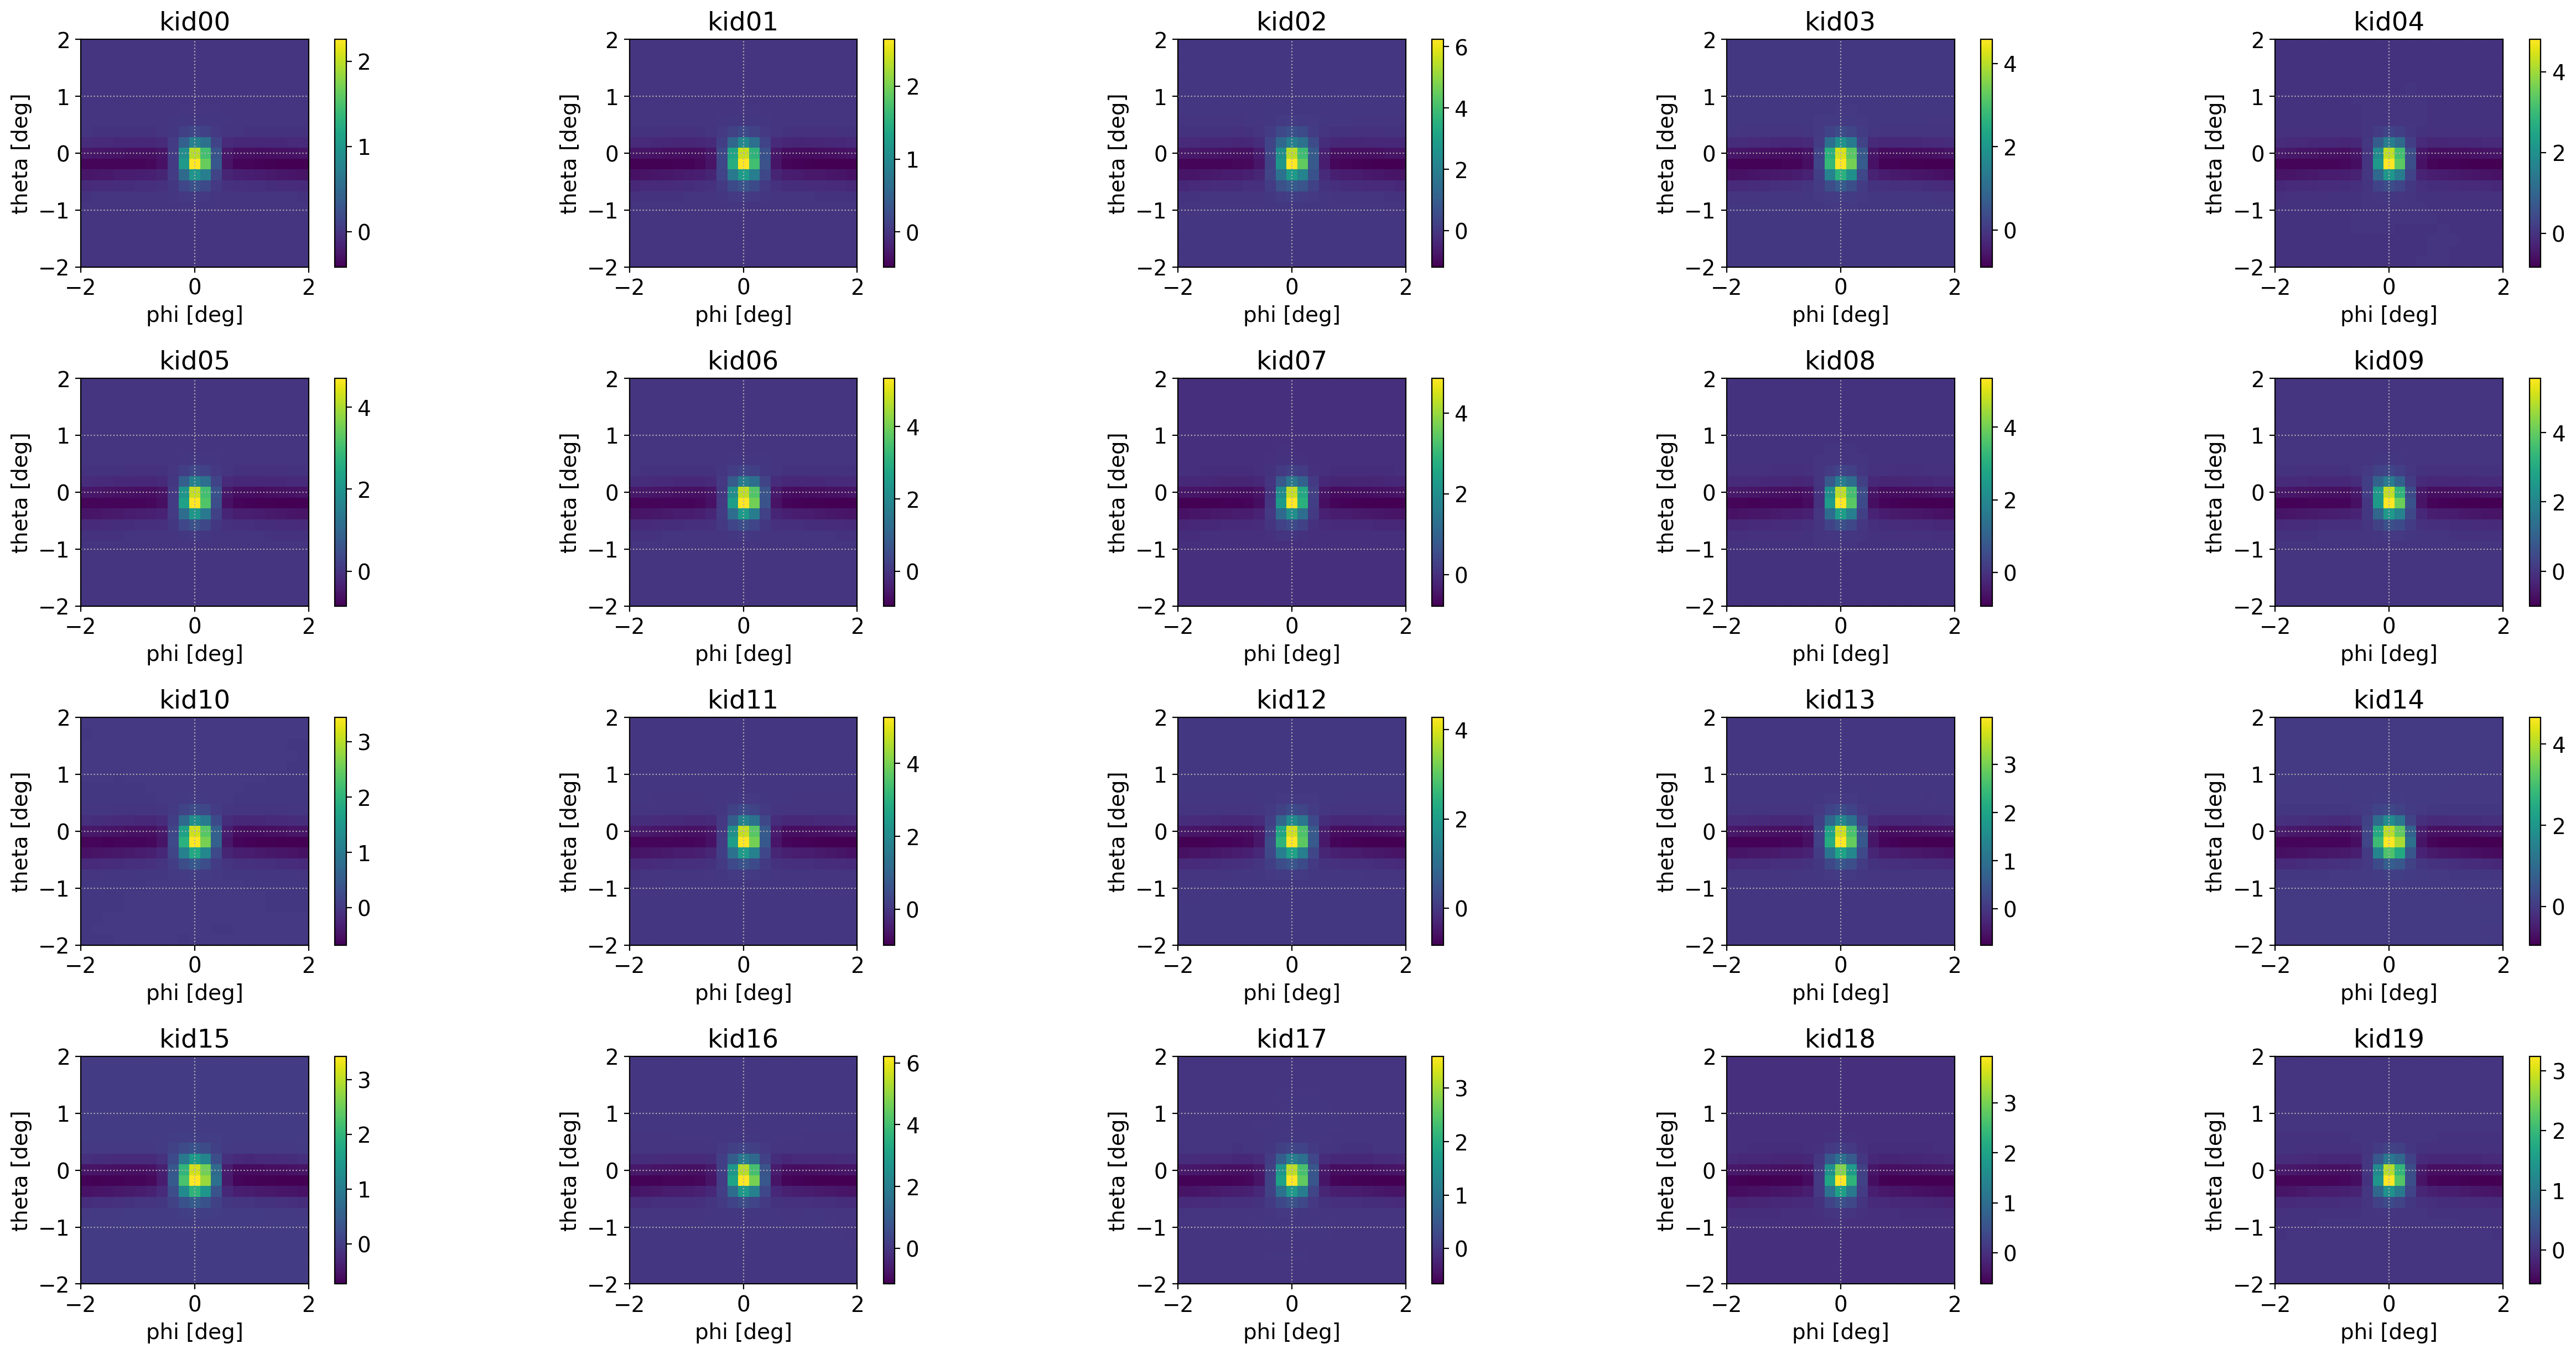
\includegraphics[width=0.85\columnwidth]{5_alignment/figs/moon_centered_6550.png}
  \caption{各MKIDの月中心マップ。座標中心(月中心)で位相が高くなる。}
  \label{moon_centered_6550}
\end{figure}

次にこの月中心のマップから各検出器が見ている空(視線)の情報を取得する。月中心マップでは検出器を個別に見ていたが、検出器全体としての視線情報を得るには望遠鏡の視線中心、つまりビームを中心とした時にどの位置で月を観測したかを知る必要がある。そのため、\SI{220}{GHz}アレイの中心にある検出器(kid17とラベルした)をビーム中心と考え、このビーム中心に対する月のマップを構成した。構成したマップの中で位相が最大となる位置を月の中心を見ていた位置として視線の代表点とする。\SI{220}{GHz}アレイのビーム中心マップと視線のプロットを図\ref{6550_beam_centered}に示す。
\begin{figure}[h]
  \begin{tabular}{cc}
    %---- 最初の図 ---------------------------
    \begin{minipage}[t]{0.48\hsize}
      \centering
      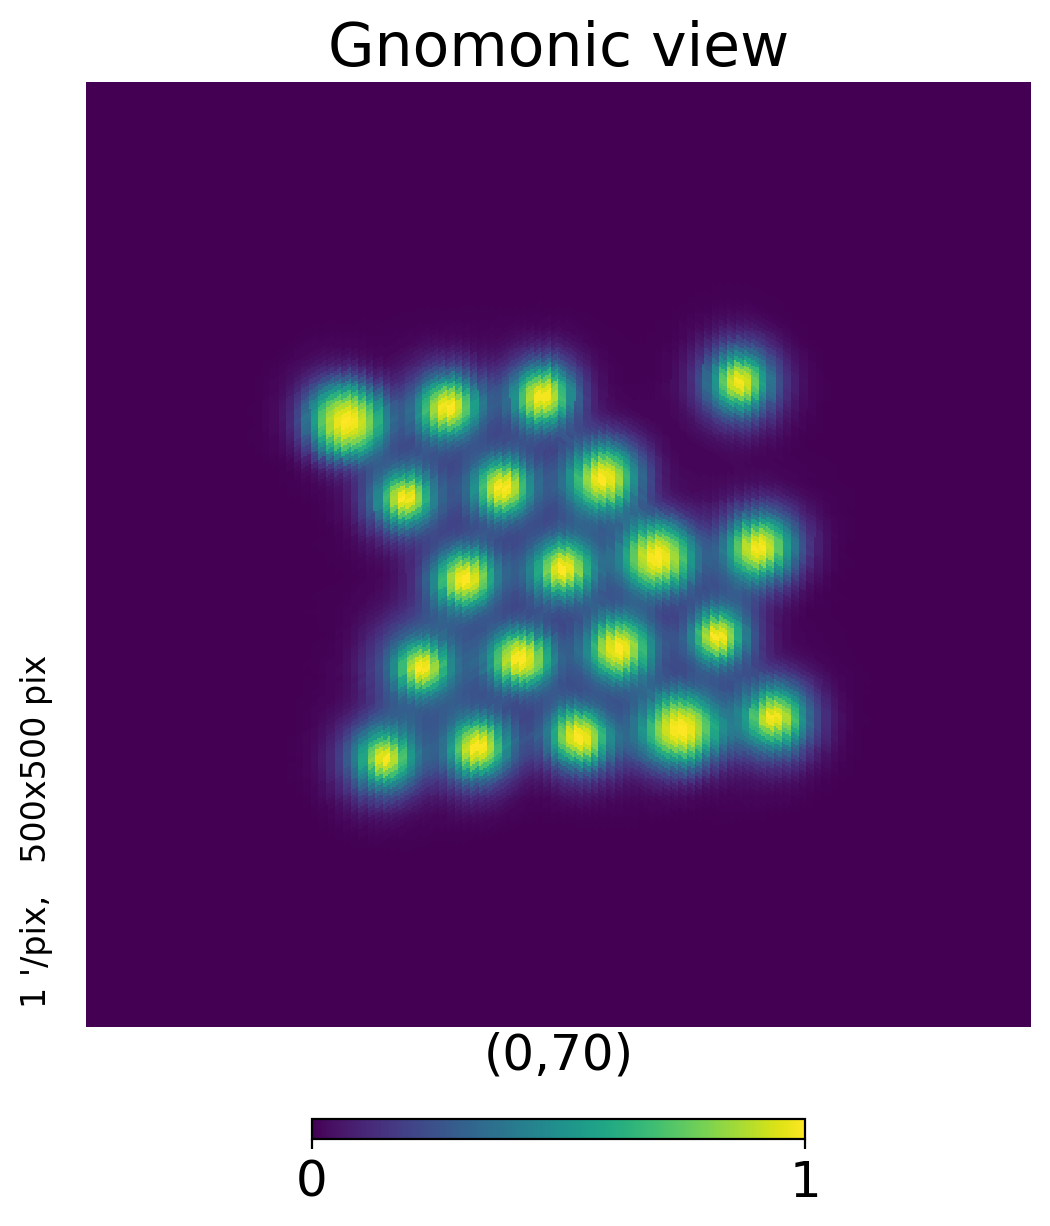
\includegraphics[keepaspectratio, scale=0.4]{5_alignment/figs/6550_gnomonic.png}
      \subcaption{\SI{220}{GHz}アレイのビーム中心マップ。}
      \label{6550_gnomview}
    \end{minipage}
    %---- 2番目の図 --------------------------
    \begin{minipage}[t]{0.48\hsize}
      \centering
      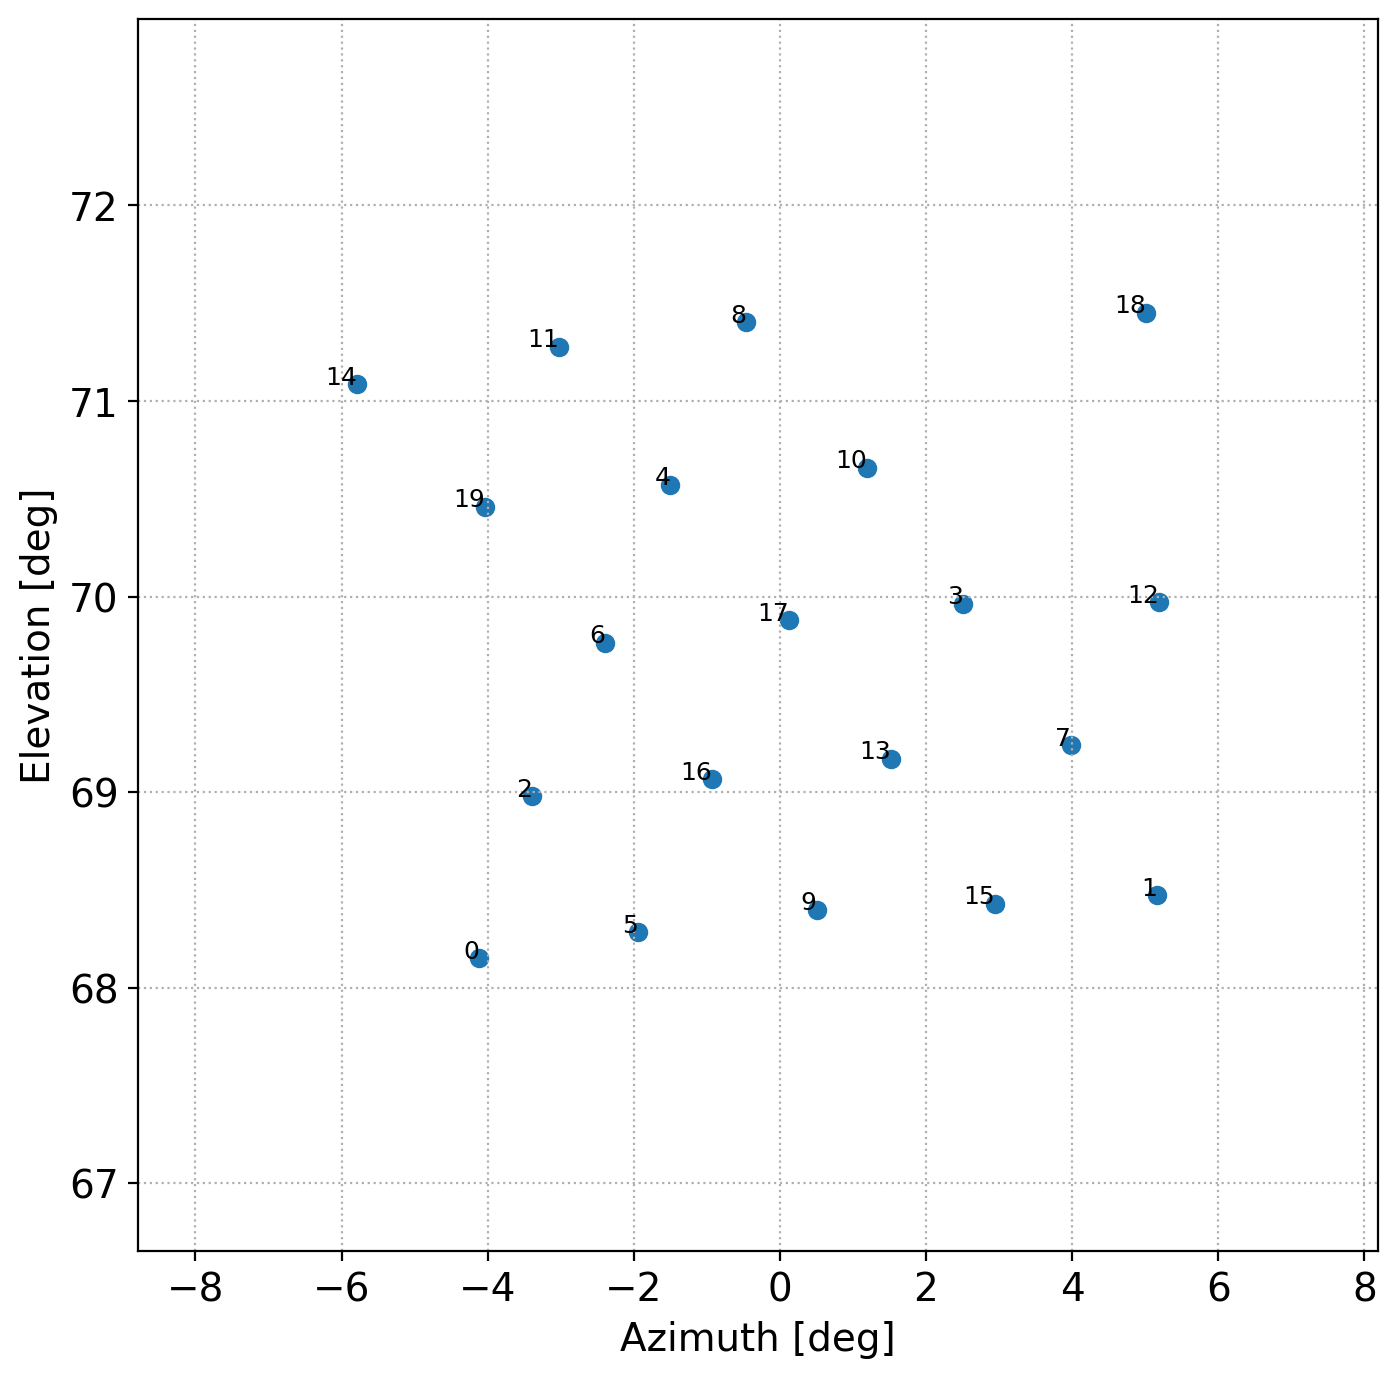
\includegraphics[keepaspectratio, scale=0.32]{5_alignment/figs/6550_pos_kid17_70.png}
      \subcaption{各検出器のビーム中心の視線。}
      \label{6550_pos}
    \end{minipage}
    %---- 図はここまで ----------------------
  \end{tabular}
  \caption{ビーム中心マップから取得した検出器の視線}
  \label{6550_beam_centered}
\end{figure}
ここで\ref{6550_gnomview}では``healpy\cite{healpy}''のgnomviewを使って球面のマップを平面射影している。また、\ref{6550_pos}には検出器のラベルとして各点に番号を記した。この図から検出器の配置がスキャン軸に対して傾いていることが見て取れる。また、中心アレイでは仰角$\SI{70}{^{\circ}}$でも球面による歪みが少なく平面的に見えている。

加えて中心以外の\SI{145}{GHz}アレイも含めた検出器全体でのビーム中心マップを見て傾きを確認した。TODは同時刻帯の月を観測した時のものを使用した。使用データを表\ref{before_full_array_table}に示す。
\begin{table}[htbp]
  \centering
  \caption{ビーム中心マップの構成に使用した月観測データ}
  \vspace{3mm}
  \begin{tabular}{cccc} \hline
    観測日(UTC) & 観測時間 [min] & 周波数 [GHz] & 月の昇降(rise or set) \\ \hline
    2024/2/22 0:04 - 1:04 & 60 & 145 & set \\
    2024/2/22 0:17 - 1:17 & 60 & 145 & set \\
    2024/2/22 0:18 - 1:18 & 60 & 145 & set \\
    2024/2/22 0:37 - 1:37 & 60 & 220 & set \\
    2024/2/22 0:48 - 1:48 & 60 & 145 & set \\
    2024/2/22 0:48 - 1:48 & 60 & 145 & set \\
    2024/2/22 1:10 - 2:10 & 60 & 145 & set \\ \hline

  \end{tabular}
  \label{before_full_array_table}
\end{table}
ビーム中心マップと全検出器の視線は図\ref{6550_beam_centered}と同じ計算で求めた(図\ref{before_full_beam_map}と図\ref{before_full_beam_pos})。
%\begin{figure}[h]
  %\begin{tabular}{cc}
    %---- 最初の図 ---------------------------
    %\begin{minipage}[t]{0.48\hsize}
      %\centering
      %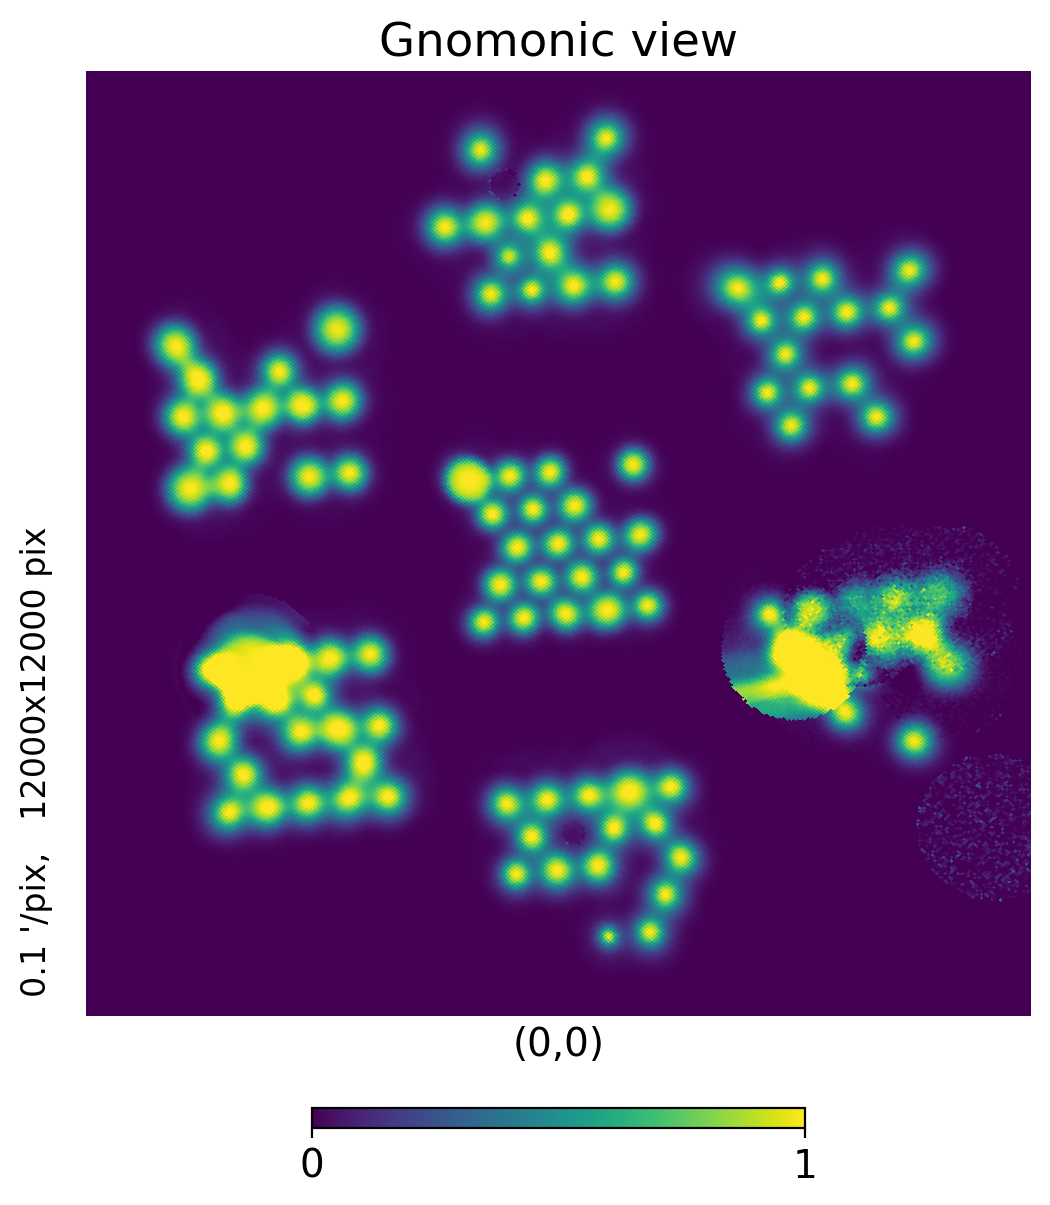
\includegraphics[keepaspectratio, scale=0.4]{5_alignment/figs/before_full_gnomonic.png}
      %\subcaption{フルアレイのビーム中心マップ。}
      %\label{before_full_beam_map}
    %\end{minipage}
    %---- 2番目の図 --------------------------
    %\begin{minipage}[t]{0.48\hsize}
      %\centering
      %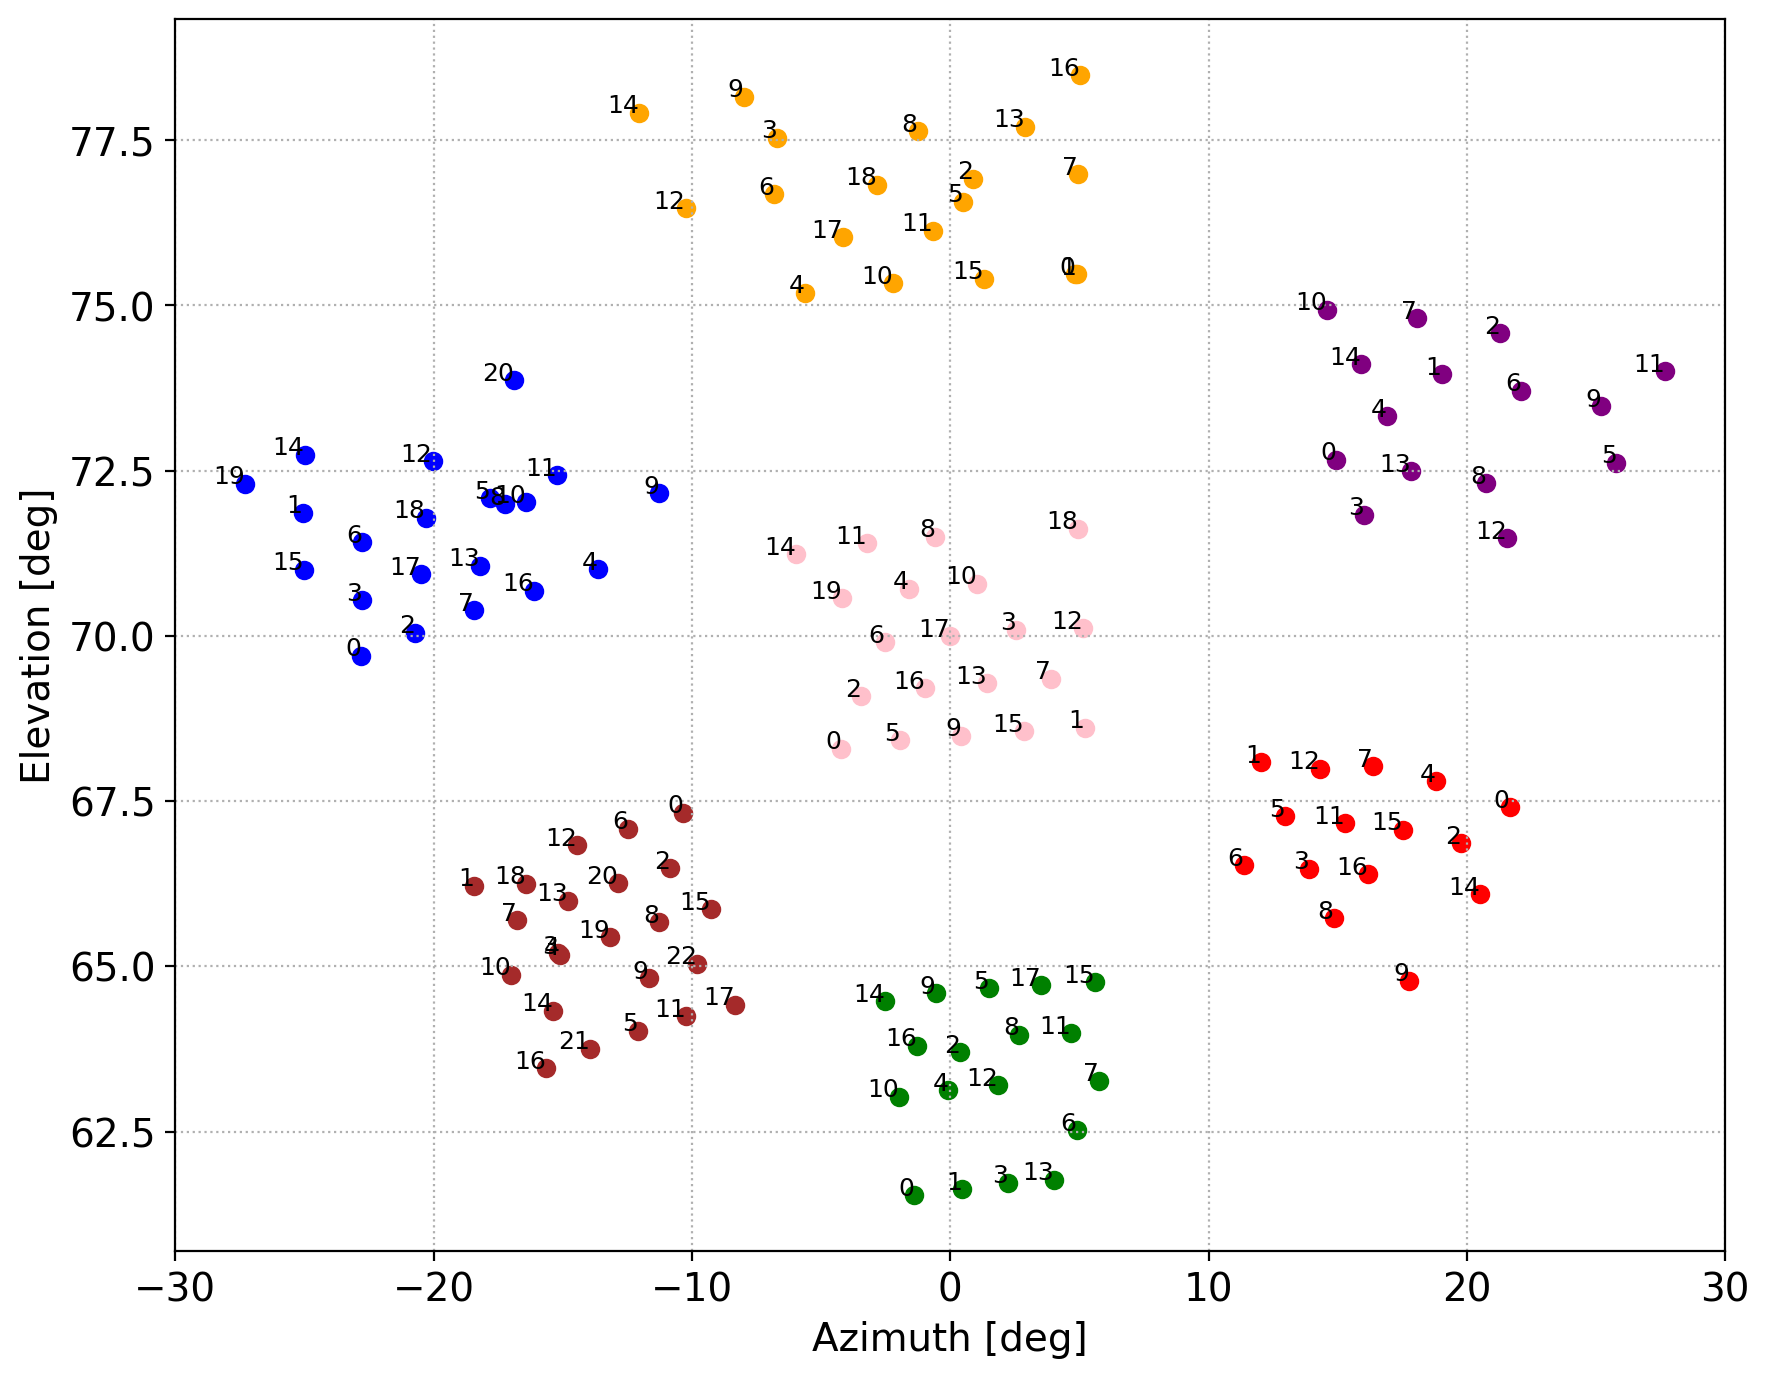
\includegraphics[keepaspectratio, scale=0.32]{5_alignment/figs/before_full_pos_70.png}
      %\subcaption{全検出器のビーム中心の視線。}
      %\label{before_full_pos_70}
    %\end{minipage}
    %---- 図はここまで ----------------------
  %\end{tabular}
  %\caption{ビーム中心マップから取得した全検出器の視線}
  %\label{before_full_beam_centered}
%\end{figure}
\begin{figure}[htbp]
  \centering
  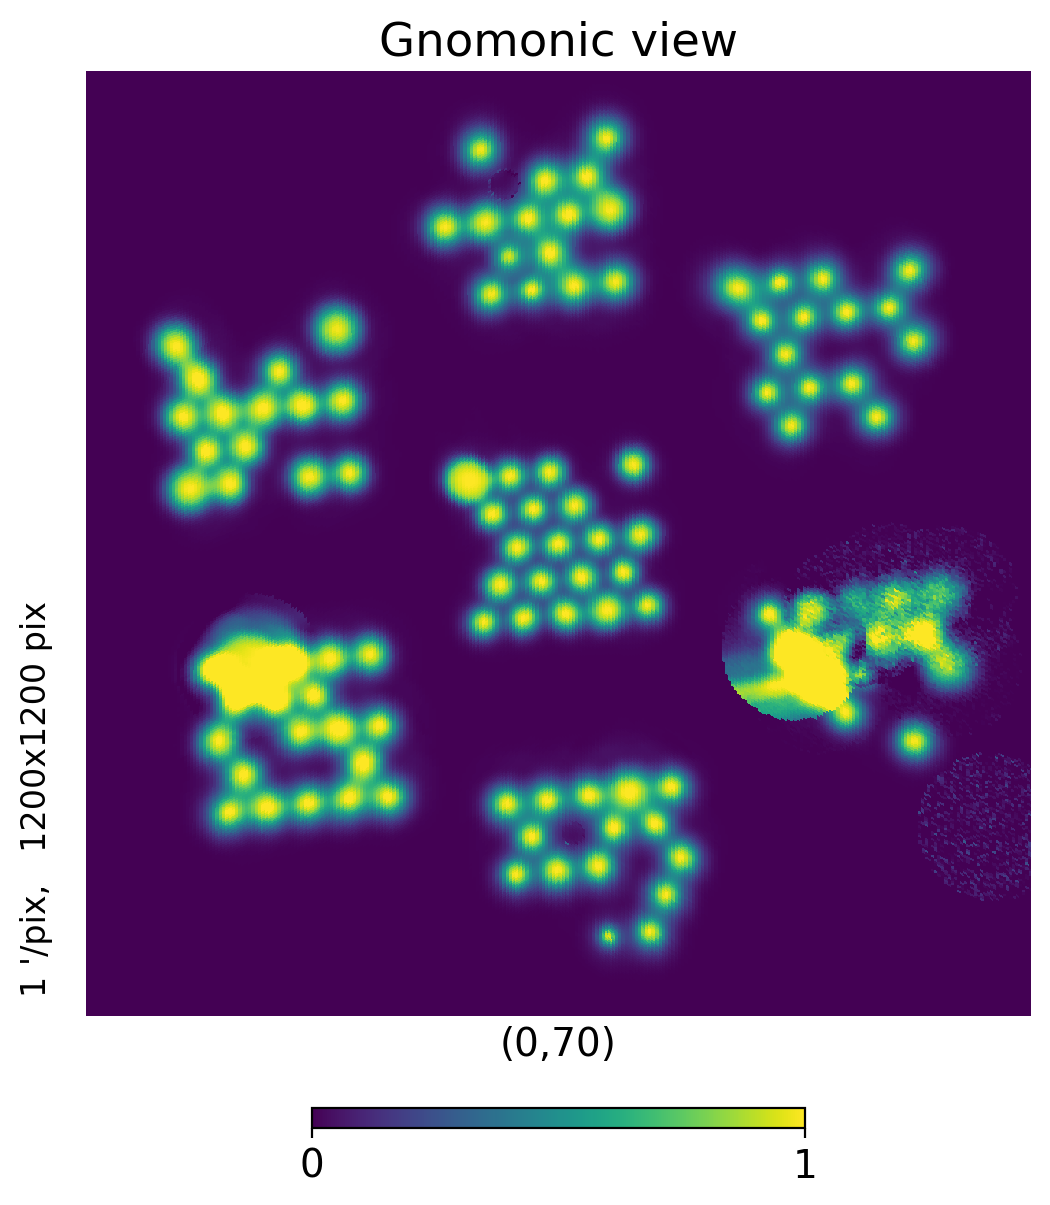
\includegraphics[width=0.7\columnwidth]{5_alignment/figs/before_full_gnomonic_70.png}
  \caption{フルアレイのビーム中心マップ。}
  \label{before_full_beam_map}
\end{figure}
\begin{figure}[htbp]
  \centering
  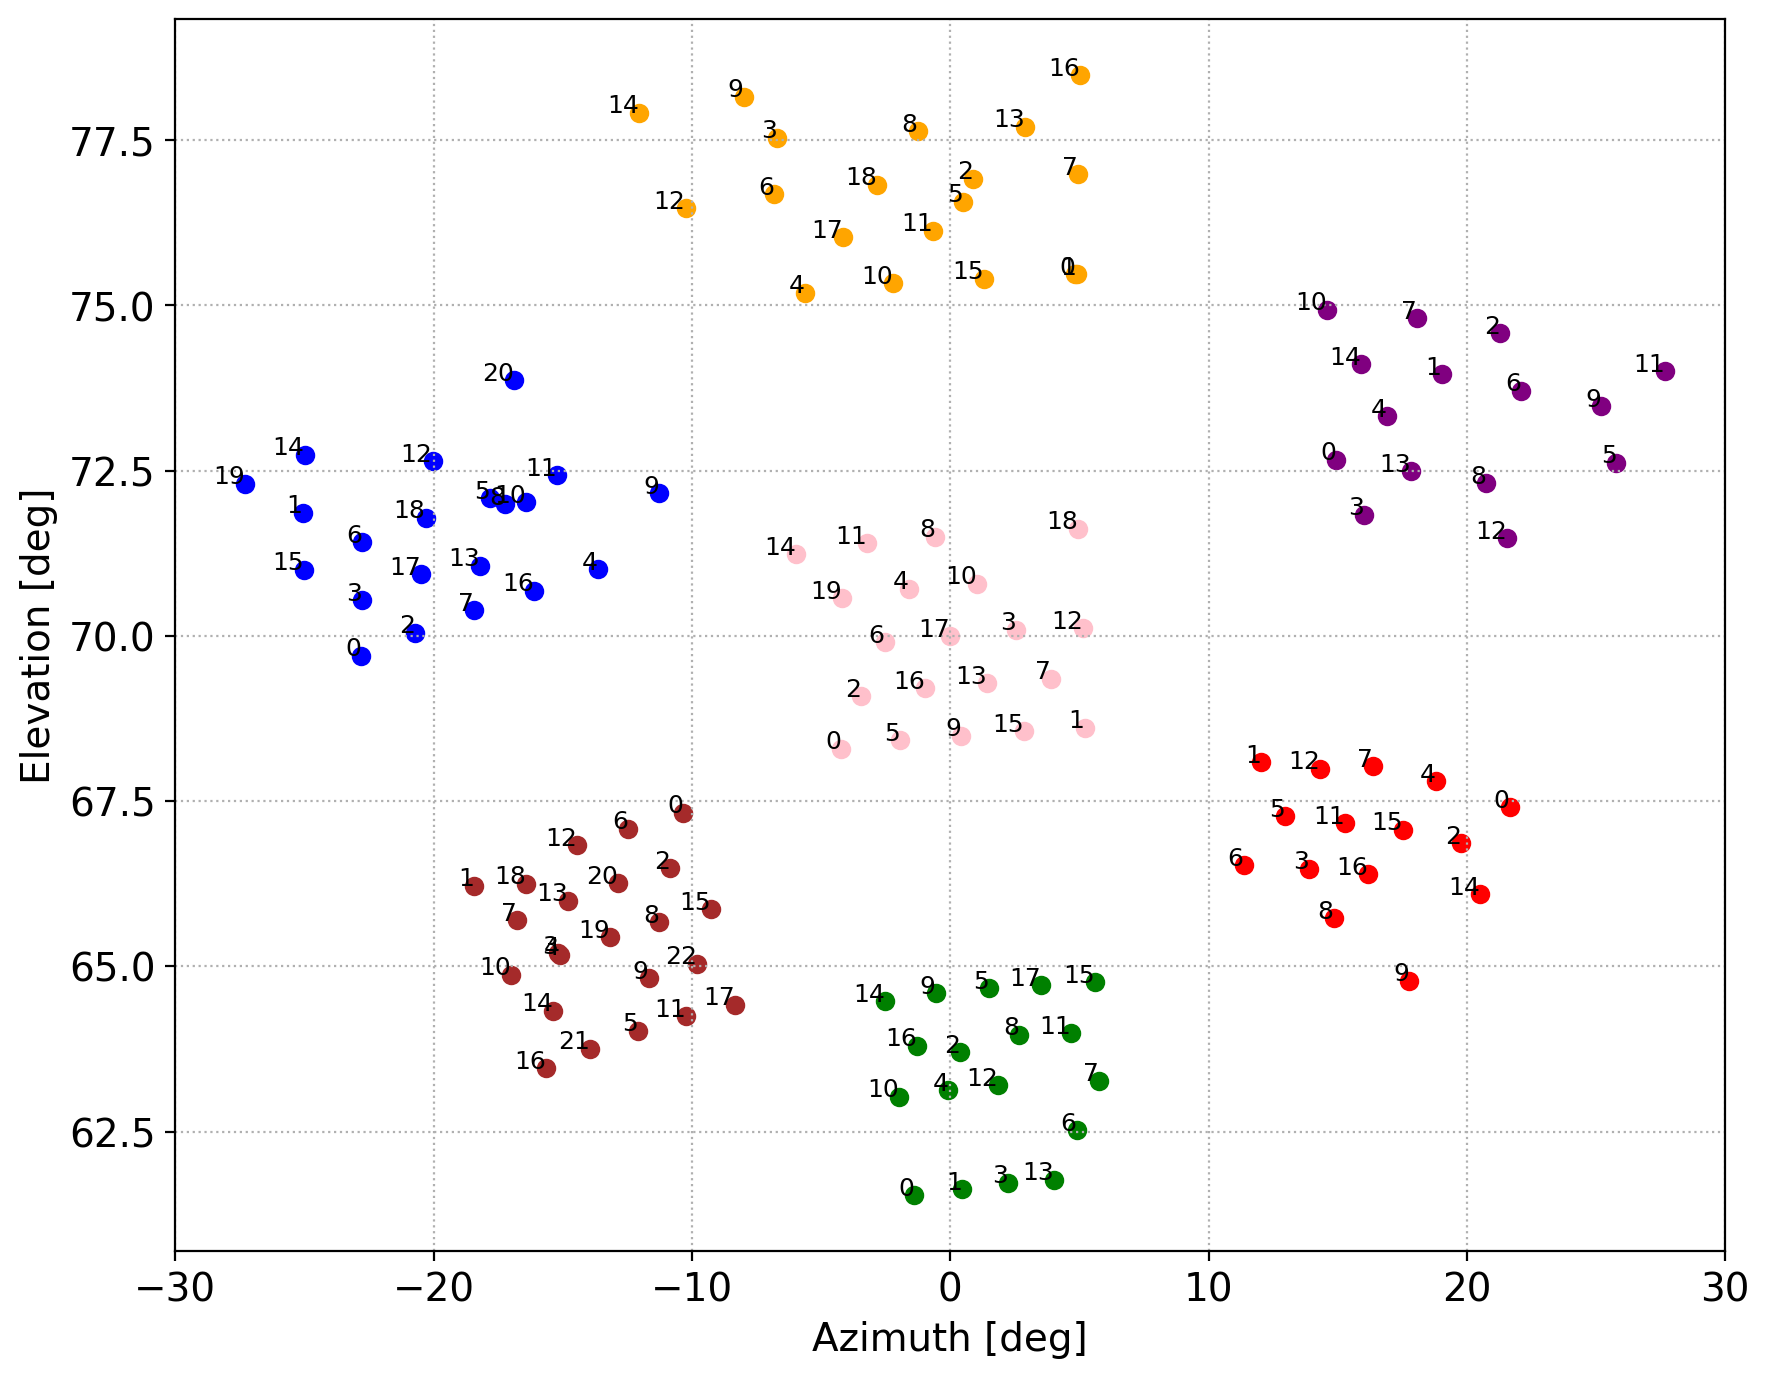
\includegraphics[width=1.0\columnwidth]{5_alignment/figs/before_full_pos_70.png}
  \caption{全検出器のビーム中心の視線。}
  \label{before_full_beam_pos}
\end{figure}

\subsection{回転する上でのジグの必要性}

\section{ジグの設計と現地インストール}

\subsection{固定用ジグの作成}

\subsection{望遠鏡への実装}

\section{天体を用いた較正結果の確認}

\subsection{月データによる確認}

\subsection{木星データによる確認}
\label{jupiter_ana}

\section{検出器間差分で見る大気揺らぎの抑制}

\subsection{timing offsetの算出}

\subsection{差分解析による確認}
